% metadata{{{
\begin{filecontents*}{\jobname.xmpdata}
\Title{User manual for AnalysisTools}
\Author{Karel Šindelka}
\Keywords{}
\Publisher{}
\end{filecontents*} %}}}
\documentclass[12pt,a4paper]{report}
% pagesize %{{{
\setlength\textwidth{145mm}
\setlength\textheight{230mm}
\setlength\oddsidemargin{0mm}
\setlength\evensidemargin{0mm}
\setlength\topmargin{0mm}
\setlength\headheight{0mm} %}}}

%\usepackage{layouts}
% used packages %{{{
% create pdf/a-2u
%\usepackage[a-2u]{pdfx}
% utf8 encoding
\usepackage[utf8]{inputenc}
% paper size
\usepackage[lmargin=3cm,rmargin=3cm]{geometry}
% to include images
\usepackage{graphicx}
% math stuff
\usepackage{amsmath}
% for customizing array fields (such as include \displaystyle in column
% definitions)
\usepackage{array}
% table customization
\usepackage{multirow}
% exactly what it says on the tin - table spanning pages
\usepackage{longtable}
% better tables
\usepackage{booktabs}
% for hack to make \cline and \cmidrule work with czech babel
\usepackage{etoolbox}
% used language -- last one is the main language
\usepackage[czech,english]{babel}
% custom colours
\usepackage{xcolor}
% custom headers and footers -- replaces fancyhdr
\usepackage{titleps}
% to label subfigures
\usepackage[labelformat=empty]{subcaption}
% compress citations into [a-z]
\usepackage{cite}
% list customization
\usepackage{enumitem}
% clickable links -- hyperref should be the last package listed
\usepackage{hyperref} %}}}

% change enumerate numbering from 1. to (1)
\renewcommand\labelenumi{(\theenumi)}

% makes \cline and \cmidrule work with czech babel
\preto\tabular{\shorthandoff{-}}

% math commands %{{{
% shorten math bold command
\newcommand{\mb}{\mathbf}
% shorten math roman command
\newcommand{\mr}{\mathrm} %}}}

% define colors %{{{
\definecolor{dark-green}{rgb}{0,0.7,0}
\definecolor{dark-red}{rgb}{0.8,0,0}
\definecolor{dark-blue}{rgb}{0,0,0.9} %}}}

% blue equation links -- amsmath package %{{{
\colorlet{linkequation}{dark-blue}
\newcommand*{\SavedEqref}{}
\let\SavedEqref\eqref
\renewcommand*{\eqref}[1]{%
  \begingroup
    \hypersetup{
      linkcolor=linkequation,
      linkbordercolor=linkequation,
    }%
    \SavedEqref{#1}%
  \endgroup
} %}}}

% define headers and footers %{{{
\newpagestyle{main}{
  \setheadrule{.4pt}% Header rule
  %\setfootrule{.4pt}% Footer rule
  \sethead[\thesection. \sectiontitle]% odd-left
          []% odd-center
          [\thechapter. \chaptertitle]% odd-right
          {\thechapter. \chaptertitle}% even-left
          {}% even-center
          {\thesection. \sectiontitle}% even-right
  \setfoot[]% odd-left
          [\thepage]% odd-center
          []% odd-right
          {}% even-left
          {\thepage}% even-center
          {}% even-right
        } %}}}

\hypersetup{colorlinks, linkcolor={dark-red}, citecolor={dark-green}}

% chapter headers without too much white space %{{{
\makeatletter
\def\@makechapterhead#1{
  {\parindent \z@ \raggedright \normalfont
   \vspace*{30pt}
   \Huge\bfseries \thechapter. #1
   \par\nobreak
   \vskip 20\p@
}}
\def\@makeschapterhead#1{
  {\parindent \z@ \raggedright \normalfont
   \Huge\bfseries #1
   \par\nobreak
   \vskip 20\p@
}}
\makeatother %}}}
% macro to put unnumbered chapter to toc %{{{
\def\chapwithtoc#1{
\chapter*{#1}
\addcontentsline{toc}{chapter}{#1}
} %}}}

% number subsubsection
\setcounter{secnumdepth}{2}
% add subsubesctions to toc
\setcounter{tocdepth}{2}

% more reasonable figure placing
\setcounter{topnumber}{2}
\setcounter{bottomnumber}{2}
\setcounter{totalnumber}{4}
\renewcommand{\topfraction}{0.9}
\renewcommand{\bottomfraction}{0.8}
\renewcommand{\textfraction}{0.07}
\renewcommand{\floatpagefraction}{0.7}

\begin{document}

% some better(?) word splitting settings %{{{
\lefthyphenmin=2
\righthyphenmin=2 %}}}

\begin{center}
\thispagestyle{empty}
\textcolor{white}{.}
\vfill
\vfill
\vfill
{\Huge\bf AnalysisTools user manual}
\vfill
{\Large Karel Šindelka}

{\small k.sindelka@gmail.com}
\vspace{10pt}

\today
\vfill
\vfill
\vfill
\vfill
\vfill
\vfill
\end{center}

\pagestyle{main}
\tableofcontents

\setcounter{page}{1}
\addcontentsline{toc}{chapter}{Contents}

\chapter{Introdution}

This software package is a set of utilities aimed to analyse trajectories
of coarse-grained simulations. It works with
\href{https://github.com/olenz/vtfplugin/wiki/VTF-format}{vtf trajectory
files}.

The emphasis is mainly on assembly of molecules, e.g., self-assembly of
polymers. It therefore includes utilities to determine if molecules are in
aggregates and to calculate various properties of aggregates. Also,
throughout the utilities and this manual, the term aggregates refers to any
supramolecular structure (e.g., a bilayer, a micelle, or a vesicle).  The
package also contains some utilities to generate initial configurations (or
adapt existing configurations) as well as to create input files for the
\href{https://lammps.sandia.gov/}{LAMMPS molecular dynamic simulator} and
the
\href{https://www.scd.stfc.ac.uk/Pages/DL_MESO.aspx}{DL\_MESO
simulation package}.

\chapter{Installation} \label{chap:Install}

All programs can be compiled on linux using \texttt{cmake}, which generates
\texttt{Makefile}, and subsequently running \texttt{make}. It requires
\texttt{C} and \texttt{FORTRAN} compilers.

The compilation should be done in a separate directory, such as
\texttt{\$ROOT\_DIR/build} (\texttt{\$ROOT\_DIR} is the
\texttt{AnalysisTools} root directory). To create the \texttt{Makefile},
simply run \texttt{cmake \$ROOT\_DIR} in the \texttt{build} directory.  All
utilities are then compiled by running \texttt{make} without any arguments.
To compile individual utilities, run \texttt{make <utility name>}.
The binaries will be in \texttt{build/bin} directory.

Following is a one line command to create the \texttt{build} directory and
compile all utilities (assuming the working directory is AnalysisTools root
directory):

\texttt{mkdir build; cd build; cmake ../; make}

\chapter{Format of input/output files}\label{chap:input}

This section describes several file types used by many of the
AnalysisTools utilities. Output files for the utilities themselves are
described in their respective sections in Chapter~\ref{chap:Utils}.

Generally, the utilities work with
\href{https://github.com/olenz/vtfplugin/wiki/VTF-format}{vtf files} which
are convenient text files containing particle coordinates as well as
particle definitions (name, mass, charge, etc.) and molecule connectivity
(i.e., bonds between particles). Additional information (e.g., bond angles
or dihedrals) can be added from other sources such as input files for
\href{https://www.scd.stfc.ac.uk/Pages/DL_MESO.aspx}{DL\_MESO simulation
package} or \href{https://lammps.sandia.gov/}{LAMMPS molecular dynamics
simulator}.

\section{System description} %{{{
Most of the utilities read system description from the \vtf files
which can be complemented by a DL\_MESO \field or a LAMMPS \data files. Not
all valid \vtf files will work with AnalysisTools; see the following
sections for information their proper formatting

The \vtf can either be split into a \vsf structure file
(Section~\ref{ssec:StructureVsf}) and a \vcf coordinate file
(Section~\ref{ssec:CoordinateVcf}), or presented in a single \vtf file
containing both the structure and coordinate sections; note that when
individual \vscf files are mentioned in the manual, they can usually be
viewed as \vscf sections of the combined \vtf file. The advantage of using
separate structure and coordinate files is that the same coordinate file
can sometime be used with different structure files to get different
results.

In general, the utilities consider only bead types that are present in a
\vcf file (i.e., bead types present in a \vsf file but missing from a \vcf
file are ignored).

Some of the utilities work with orthogonal as well as other paralleloid
boxes (i.e., triclinic cells).

\subsection{\vsf structure file} \label{ssec:StructureVsf} %{{{

The structure file contains all information about all beads and bonds
(except for their Cartesian coordinates) in two types of entries. The first
type, an \enquote{atom line}, contains a bead definition, while the second
one, a \enquote{bond line}, defines which beads are connected.

Each atom line describes a single bead (except for the \tt{atom default}
line, see below) and must follow these rules:

\begin{itemize}[topsep=0pt,itemsep=0pt]
  \item the line starts with \tt{a[tom]} (i.e., \tt{atom} or just \tt{a})
  \item the second string is either a bead index (starting at 0) or the
    \tt{default} keyword; every bead that is not explicitly written in the
    bead definition lines is of the \tt{default} type (in case of multiple
    \tt{default} lines, the first one is used while the subsequent ones are
    ignored)
  \item the line contains bead name as \tt{n[ame] <char(16)>}
  \item if the bead is in a molecule, the line contains both molecule name
    (\tt{res[name] <char(8)>}) and molecule id (\tt{resid <int>}) starting
    at 1
  \item \tt{m[ass]}, \tt{charge|q} (i.e., \tt{charge} or \tt{q}), and
    \tt{r[adius]} keywords are read if present
  \item other keywords are ignored
\end{itemize}

Each bond line starts with \tt{b[ond]} followed by two bead indexes
(corresponding to their indexes from the atom lines) separated by a colon.
Note that the colon must be right after the first index, i.e., no white
space between the number and the colon is allowed.

\tt{AnalysisTools} groups the same beads (and the same molecules) into bead
(and molecule) types. Generally, types of beads are defined solely by their
name, i.e., should two beads share a name but differ in other
characteristics, they will be grouped into the same type with mass, charge,
and radius each equal to that for the bead type's topmost atom line with
the corresponding keyword. If the keyword is missing from all atom lines,
that characteristic is undefined. Similarly, different molecule molecules
are generally defined based on their names. If two molecules share a name,
but differ in bead order and/or connectivity, the utility will exit with an
error.

However, some utilities can distinguish bead and molecule types based on
other characteristics as well. For example, the \tt{--detailed} option
forces the \tt{Info} utility (\ref{sec:Info}) to consider mass,
charge, and radius along with the name for defining bead types and bead
order and connectivity along with the name for defining molecule types. As
an example, consider the following \vsf file that contains 11 beads and
two molecules:

...well, I wish it actually worked.

\begin{lstlisting}
atom default name A mass 1 charge 0
atom 0 name B mass 2 radius 1
atom 2 name B mass 1 charge -1
atom 4 name B
atom 5 name C resname Mol resid 1 mass 1
atom 6 name A resname Mol resid 1 mass 1
atom 7 name A resname Mol resid 1
atom 8 name C resname Mol resid 2
atom 9 name D resname Mol resid 2 radius 1.5
atom 10 name D resname Mol resid 2 mass 2
bond 5:6
bond 6:7
bond 8:9
bond 9:10
bond 8:10
\end{lstlisting}

Using \tt{Info <vsf>}, bead and molecule types are identified by their name
only:

\begin{lstlisting}
Counts = {
  .TypesOfBeads     = 4,
  .Bonded           = 6,
  .Unbonded         = 5,
  .Beads            = 11,
  .TypesOfMolecules = 1,
  .Molecules        = 2
}

BeadType[0] = {.Name = A, .Number = 4, .Charge = 0.0,
                                  .Mass = 1.0, .Radius = n/a}
BeadType[1] = {.Name = B, .Number = 3, .Charge = n/a,
                                  .Mass = 2.0, .Radius = 1.0}
BeadType[2] = {.Name = C, .Number = 2, .Charge = n/a,
                                  .Mass = 1.0, .Radius = n/a}
BeadType[3] = {.Name = D, .Number = 2, .Charge = n/a,
                                  .Mass = n/a, .Radius = 1.5}

MoleculeType[ 0] = {
  .Name       = Mol,
  .Number     = 2,
  .nBeads     = 3,
  .Bead       = {C, A, A},
  .nBonds     = 2,
  .Bond       = {1-2, 2-3},
  .nBTypes    = 2
  .BType      = {C, A},
  .Mass       = 3.0,
  .Charge     = n/a
}
\end{lstlisting}

Here, four bead types and a single molecule type are identified. Looking,
for example, at the mass of the \tt{B} beads, its value is 2 according to
the second line in the \vsf file (the first atom line containing the name
\tt{B}) even though the mass of \tt{B} on the next atom line is 1. Looking
at the single molecule type, it contains bead types \tt{C} and \tt{A}
connected \tt{C-A-A}; these were taken from the first molecule (\vsf lines
5-7). However, the second molecule is in the shape of a triangle (see \vsf
lines 13-15).

The \vsf file can contain any number of blank lines and comments (lines
beginning with \tt{\#}).

See complete examples of the \vsf file (as well as of some errors) in the
\tt{Examples} directory.

\subsection{\vcf coordinate file} \label{ssec:CoordinateVcf}

The coordinate file contains Cartesian coordinates of the beads and the
size of the paralleloid simulation box. Coordinates are read from a \vcf
file containing either ordered timesteps or indexed timesteps; all
timesteps must be of the same type and contain the same beads.

An ordered \vcf file must contain all beads defined in the \vsf file, while
an indexed \vcf file can contain only a subset of defined beads. Both
indexed and ordered \vcf files contain a line before every timestep
specifying the file type, \tt{t[imestep] o[rdered]/i[ndexed]}; the
\tt{timestep} keyword can be omitted.

In both ordered and indexed \vcf files, the size of the simulation box is
given by a line appearing before the first timestep:
%
\begin{lstlisting}
pbc <x> <y> <z> # cuboid simulation box
pbc <a> <b> <c> <alpha> <beta> <gamma> # triclinic box
\end{lstlisting}
%
Should this line also prepend other timesteps, the box dimensions are
adjusted accordingly.

The \vcf file may contain comment lines (beginning with
\tt{\#}) and blank lines between timesteps, but the coordinate block
must be continuous.

The coordinate blocks in an ordered \vcf file contain only Cartesian
coordinates -- every line has the \tt{<x> <y> <z>} format The beads are
written in an ascending order of their indices as defined in the \vsf file.
All beads defined in the \vsf file must be present in the ordered \vcf
file.

The coordinate blocks in an indexed \vcf file contain not only Cartesian
coordinates but also bead indices -- every line has the \tt{<index> <x> <y>
<z>} format. An indexed timestep does not have to contain all beads defined
in the \vsf structure file; however, \tt{AnalysisTools} utilities work with
whole sets of beads, that is, when one bead of a specific type is missing,
all beads of that type (or with the same name) must be omitted as well.
The beads do not have to be ordered in any specific way.

Velocities can also be included following the Cartesian coordinates, i.e.,
\begin{lstlisting}
<index> <x> <y> <z> <vel(x)> <vel(y)> <vel(z)>
\end{lstlisting}
 %}}}

\subsection{DL\_MESO \field file} %{{{

\begin{comment}
This file can be used to get mass and/or charge of bead types (only if
missing from the \vsf file) as well as bond parameters and angle and angle
parameters for molecules (these informations are not stored in the \vsf
file).

The format of this file is taken directly from the
\href{https://www.scd.stfc.ac.uk/Pages/DL_MESO.aspx}{DL\_MESO}
software. If the \field file is used only to read mass and/or charge
information about bead types, only the \tt{species} section is required.
This section contains a header line
\begin{verbatim}species <int>\end{verbatim}
where \tt{<int>} is the number of bead types (or species as called by the
DL\_MESO software) in the \field file. Every bead type is then describe by
a single line:
\begin{verbatim}<name> <m> <q> <n>\end{verbatim}
where \tt{<name>} is the bead type name (that must correspond to a bead
name in the \vsf file if its mass/charge is to be read from the \field
file), \tt{m} and \tt{q} are the bead's mass and charge, respectively,
and \tt{<n>} is the number unbonded beads of that type (i.e., beads
not present in a molecule). Not all bead types in the \vsf file must be
present in the \field file. Blank lines are not allowed in the \tt{species}
section.

Should bond and angle information be read as well, a \tt{molecules} section
must follow the \tt{species} section. This section starts with a header line:
\begin{verbatim}molecule <int>\end{verbatim}
where \tt{<int>} is the number of types of molecules. The header is
followed by \tt{<int>} blocks, each describing a single molecule type and
ending with a line:
\begin{verbatim}finish\end{verbatim}
Every molecular block starts with two lines:
\begin{verbatim}<name>
nummols <n>\end{verbatim}
where \tt{<name>} is the molecule's name (that must correspond to a
\tt{resname} in the \vsf file if the bond/angle information is to be read)
and \tt{<n>} is the number of molecules of this type (that does not have to
correspond to the number of \tt{<name>} molecules in the \vsf file).

The rest of the molecule's description is divided into several sub-blocks:
(i) bead order and coordinates, (ii) bond connectivity, and (iii) angles
which is optional. Bead order as well as connectivity must correspond to
that of the \tt{<name>} molecule in the \vsf file.

Block (i) starts with a line:
\begin{verbatim}beads <beads>\end{verbatim}
where \tt{<beads>} is the number of beads in the molecule. Following are
\tt{<beads>} lines for each bead:
\begin{verbatim}<name> <x> <y> <z>\end{verbatim}
where \tt{<name>} is a bead name that must be present in the \tt{<species>}
section and \tt{<x>}, \tt{<y>}, and \tt{<z>} are Cartesian coordinates.

Block (ii) starts with a line:
\begin{verbatim}bonds <n>\end{verbatim}
where \tt{<n>} is the number of bonds in the molecule. Following are
\tt{<n>} lines for each bond:
\begin{verbatim}harm <l> <m> <k> <r>\end{verbatim}
where \tt{<l>} and \tt{<m>} are bead indices of connected beads that run
from 1 to \tt{<beads>} and \tt{<k>} and \tt{<r>} are the strength and
equilibrium distance, respectively, of a harmonic oscillator (AnalysisTools
assumes bonds use harmonic potential).

Block (iii) starts with a line:
\begin{verbatim}angles <n>\end{verbatim}
where \tt{<n>} is the number of angles in the molecule. Following are
\tt{<n>} lines for each angle:
\begin{verbatim}harm <l> <m> <n> <k> <alpha>\end{verbatim}
where \tt{<l>}, \tt{<m>}, and \tt{<n>} are bead indices defining the angle
that run from 1 to \tt{<beads>} and \tt{<k>} and \tt{<alpha>} are the
strength and equilibrium angle, respectively, of a harmonic oscillator
(AnalysisTools assumes angles use harmonic potential). This block is optional.

Anything between the last angle line and the \tt{finish} keyword is ignored.

Several examples of a \field file can be found in the \tt{Examples}
directory, e.g., in \tt{Examples/AddToSystem}.
\end{comment}
 %}}}

\subsection{LAMMPS \data file} %{{{
 %}}}
  %}}}

\section{Aggregate file (\tt{agg})} \label{ssec:AggFile} %{{{

A \tt{file.agg} is generated using
\tt{Aggregates} (or \tt{Aggregates-NotSameBeads}) utility. The
file contains information about the number of aggregates in each timestep
and which molecules and monomeric (i.e., unbonded) beads belong to which
aggregate. It serves as an additional input file for utilities that
calculate aggregate properties; \tt{agg} file is, therefore, linked to
the \vcf file that was used to generate it.

The \tt{agg} file is a simple text file. The first line contains the
command used to generate it -- parts of this command may be necessary for
subsequent analysis of aggregates. The second line is blank, and from the
third line, the data for individual timesteps are shown. It follows these
rules:

\begin{itemize}[topsep=0pt,itemsep=0pt]
  \item each timestep starts with \tt{Step: <int>} (only \tt{Step}
    keyword is read by the utilities)
  \item the second line is the number of aggregates in the given
    timestep and is followed by a blank line
  \item there are two lines for each aggregate:
  \begin{enumerate}[topsep=0pt,itemsep=0pt]
    \item number of molecules in the aggregate followed by their indices
      taken from the \vsf file (\tt{resid} indices)
    \item number of monomeric beads in the aggregate followed by their
      indices taken from the \vsf file (\tt{atom} indices)
  \end{enumerate}
  \item no blank or comment lines are allowed inside the aggregate block
  \item not all molecules present in the \vcf file used to generate
    this file must be present in every timestep
\end{itemize}

Note that the term aggregate also refers to free chains (i.e., fully
dissolved chains).

When the keyword \tt{Last} is present instead of \tt{Step}, it
signalises the end of the \tt{agg} file; no utility will read anything
beyond this keyword.

Besides using this file for further analysis by other utilities, the
indices can be used in \href{http://www.ks.uiuc.edu/Research/vmd/}{vmd} to
visualize, e.g., only a specific aggregate by using \tt{resid 1 2 3} in the
\tt{Selected Atoms} box in vmd.

An example of an \tt{agg} file can be found in the \tt{Examples/DistrAgg}
directory. %}}}

\chapter{Utilities} \label{chap:Utils}

All utilities have command line help with short description when
\texttt{-h} argument is used. Besides \texttt{-h}, most of the utilities
have several standard command line options that are the same. The standard
options can be used with any utility unless stated otherwise.

\vspace{1em}
\noindent
\begin{tabular}{p{0.14\textwidth}p{0.804\textwidth}}
  \toprule
  \multicolumn{2}{l}{Standard options} \\
  \midrule
  \texttt{-i <name>} & use custom \texttt{vsf} file instead of
    \texttt{traject.vsf} \\
  \texttt{-v}        & verbose output that provides information about all
    bead and molecule types \\
  \texttt{-V}        & detailed verbose output that provides
    information about all individual molecules as well as about bead and
    molecule types \\
  \texttt{-s}        & run silently, i.e., without any output at all
    (overrides \texttt{-v} and \texttt{-V} options) \\
  \texttt{--script}  & do not rewrite terminal line (useful if output is
    routed to a file) \\
  \texttt{-h}        & print help and exit \\
  \bottomrule
\end{tabular}

\section{Angle Molecules} \label{sec:AngleMolecules}

This utility calculates angles (distribution and overall averages) between beads
in each molecule of specified molecule type(s); the input structure file must
contain angles (such as LAMMPS \data file). It can also calculate angles between
any three beads in the molecule type(s) via the \tt{-n} option. See
\tt{Examples/AngleMolecules} for an example.

By default, the angles are calculated for every molecule type, but the \tt{-m}
option can be used to specify only some of them.

The utility groups angles according to bead types; e.g., in a linear 6-bead
molecule (such as in the \tt{Example/AngleMolecules} directory) with bead order
A-A-A-B-A-A with all possible angles defined (i.e., 1-2-3, 2-3-4, 3-4-5, and
4-5-6 where the numbers specify bead indices in the molecule), there are three
angle types: A-A-A, A-A-B, and A-B-A. However, using the \tt{--all} option, all
molecular angles are averaged separately as well; i.e., beside for the three
angles based on bead types, the distributions and averages are calculated for
all five angles in the molecule too.

Using \texttt{-n} option, extra angles are specified by three bead indices taken
from the bead order in the molecule type(s). These indices go from 1 to $N$,
where $N$ is the number of beads in the molecule type (\tt{Info} utility can be
used to check the indices). Multiple angles may be specified, and the results
are written to the specified file. Angles containing an index number that is
higher than the number of beads in a molecule are ignored only for that
molecule.

\vspace{1em}
\noindent
Usage: \tt{AngleMolecules <input> <width> <output> [options]}
\noindent
\begin{longtable}{p{0.24\textwidth}p{0.704\textwidth}}
  \toprule
  \multicolumn{2}{l}{Mandatory arguments} \\
  \midrule
  \texttt{<input>}       & input coordinate file\\
  \texttt{<width>}       & width of each distribution bin\\
  \texttt{<output>}      & output file for distribution\\
  \midrule
  \multicolumn{2}{l}{Options}\\
  \midrule
  \texttt{-m <name(s)>} & specify molecule type(s) to use\\
  \texttt{--joined}     & specify that \texttt{<input>} contains joined
    coordinates\\
  \texttt{--all}        & write all angles for the molecule types\\
  \texttt{-n <file> <ints>} & multiple of three indices for extra angle\\
  \midrule
  \multicolumn{2}{l}{Other options (see the beginning of
                     Chapter~\ref{chap:Utils})}\\
  \midrule
  \multicolumn{2}{p{0.948\textwidth}}{\tt{-st},
                                      \tt{-e},
                                      \tt{-sk},
                                      \tt{-i},
                                      \tt{--verbose},
                                      \tt{--silent},
                                      \tt{--help},
                                      \tt{--version}}\\
  \bottomrule
\end{longtable}

\noindent
Format of output files:
\begin{enumerate}[nosep,leftmargin=20pt]
  \item \texttt{<output>} -- distribution of angles (grouped by bead types and
    possibly for all molecular angles as well if \tt{--all} option is used)
    \begin{itemize}[nosep,leftmargin=5pt]
      \item first line: AnalysisTools version
      \item second line: command used to generate the file
      \item following lines (number of specified molecules plus 1): column
        headers
        \begin{itemize}[nosep,leftmargin=10pt]
          \item first column is the centre of each bin in angles (governed by
            \texttt{<width>}); i.e., if \texttt{<width>} is 5$^{\circ}$,
            then the centre of bin 0 to 5$^{\circ}$ is 2.5, centre of bin 5
            to 10$^{\circ}$ is 7.5 and so on
          \item the rest are for the calculated data: for each specified
            molecule there are angles grouped by bead types followed by all
            angles in that molecule (if \tt{--all} option is used)
        \end{itemize}
      \item next lines: the calculated data
      \item last several lines (number of specified molecules plus 2): minimum,
        maximum, and arithmetic mean for each calculated angle (last line) and
        headers (preceding lines)
    \end{itemize}
  \item \texttt{-n <file>} -- angles specified by supplied molecular indices
  \begin{itemize}[nosep,leftmargin=5pt]
    \item the file structure is the same as for the default output file
  \end{itemize}
\end{enumerate}

\section{Aggregates and Aggregates-NotSameBeads} \label{sec:Aggregates}

These utilities determine which molecules belong to which aggregates (note that
\enquote{aggregate} is used for any supramolecular structure) according to a
simple criterion: two molecules belong to the same aggregate if they share at
least a specified number of contact pairs. A contact pair is a pair of two beads
belonging to different molecules which are closer than a specified distance. The
information is written into an \tt{.agg} text file described in
Section~\ref{sec:AggFile}.

% The number of contact pairs, the distance, and bead type(s) to use for
% aggregate determination are all arguments of the utilities.  Any molecule
% type(s) can be excluded from aggregate determination (\tt{-x <mol
% name(s)>} option); they are also excluded from the output \tt{agg}
% file).  Moreover, any molecules close to specified molecule(s) can be
% excluded (\tt{-xm <mol name(s)>} option); here, \enquote{close} means
% any of the bead types used in aggregate determination is closer than
% \tt{<distance>} to any bead of the specified molecule.

Periodic boundary conditions can be removed from whole aggregates via the
\tt{-j} option; the aggregate's centre of mass is always inside the simulation
box. This is useful for visualization (an aggregate will no longer be split by
the walls of the simulation box, but it may stretch far outside the boundaries
of the box) as well as for further analysis (the other utilities do not have to
join the aggregates, possibly greatly speeding up subsequent analyses).

While the \tt{Aggregates} utility uses all possible pairs of given bead types,
\tt{Aggrega}-\tt{tes-NotSameBeads} does not use same-type pairs. For example, if
bead types \tt{A} and \tt{B} are given, \tt{Aggregates} will use all three
possible bead type pairs (i.e., \tt{A-A}, \tt{A-B}, and \tt{B-B}), but
\tt{Aggregates-NotSameBeads} will use only \tt{A-B} bead type pairs.
Fig~\ref{fig:AggCheck} illustrates the behaviour: using \tt{Aggregates ... A B}
would find one contact pair between molecules 1 and 2 and two contacts between
molecules 2 and 3, whereas \tt{Aggregates-NotSameBeads ... A B} would ignore A-A
and B-B pairs, finding no contact pair between molecules 1 and 2 and only one
between molecules 2 and 3.

\begin{figure}
  \centering
  \begin{minipage}{0.45\textwidth}
    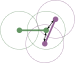
\includegraphics[scale=0.6]{AggregateCheck.jpg}
  \end{minipage}
  \begin{minipage}{0.5\textwidth}
    \tt{Aggregates ... A B}\\
    \-\hspace{30pt}$\Rightarrow$ 3 contact pairs\\
    \tt{Aggregates-NotSameBeads ... A B}\\
    \-\hspace{30pt}$\Rightarrow$ 2 contact pairs\\
  \end{minipage}
  \caption{
    Simple example of distance checks---three two-bead molecules, where dotted
    lines represent maximum pair distance (\tt{-d} option) and black arrows show
    contact pairs. Note the same bead can be a part of multiple pairs.
  }
  \label{fig:AggCheck}
\end{figure}

Note that when \tt{-st}, \tt{-e}, or \tt{-sk} options are used, the resulting
\tt{agg} file is no longer coupled to the original coordinate file (i.e., they
cannot be used together for further analyses), but it is coupled to the optional
output file with joined coordinates (\tt{-j} option).

\vspace{1em}
\noindent
Usage: \tt{Aggregates <input> <out.agg> <bead type(s)> [options]}
\noindent
\begin{longtable}{p{0.22\textwidth}p{0.724\textwidth}}
  \toprule
  \multicolumn{2}{l}{Mandatory arguments}\\
  \midrule
  \tt{<input>}        & input coordinate file\\
  \tt{<out.agg>}      & output \tt{agg} file\\
  \midrule
  \multicolumn{2}{l}{Options}\\
  \midrule
  \tt{-d <num>}       & maximum distance for contact (default: 1)\\
  \tt{-c <num>}       & minimum number of contacts (default: 1)\\
  \tt{-j <file>}      & save coordinates of joined aggregate to
                        a coordinate file\\
  \midrule
  \multicolumn{2}{l}{Other options (see the beginning of 
                     Chapter~\ref{chap:Utils})}\\
  \midrule
  \multicolumn{2}{l}{\tt{-st},
                     \tt{-e},
                     \tt{-sk},
                     \tt{-i},
                     \tt{--verbose},
                     \tt{--silent},
                     \tt{--help},
                     \tt{--version}}\\
  \bottomrule
\end{longtable}

\section{Average} \label{sec:Average}

This utility uses the binning method to analyse data in a text file. It
does not use any of the standard options and prints the result only to
standard output (e.i., screen).

\texttt{Average} calculates average, statistical error, and estimate of the
autocorrelation time $\tau$. Empty lines and comments (lines beginning with
\texttt{\#}) are skipped. \texttt{Average} prints to standard output (i.e.,
the screen) four numbers: \texttt{<n\_blocks> <average> <std error> <tau
estimate>}:
\begin{longtable}{ll}
  \toprule
  \texttt{<n\_blocks>} & number of blocks used for the binning analysis \\
  \texttt{<average>} & simple arithmetic average \\
  \texttt{<std error>} & one-$\sigma$ statistical error \\
  \texttt{<tau estimate>} & estimate of autocorrelation time $\tau$ \\
  \bottomrule
\end{longtable}

A way to quickly estimate a `real' value of $\tau$ is to use a wide range
of \texttt{<n\_blocks>} value and plot the \texttt{<tau estimate>} values
as a function of \texttt{<n\_blocks>}. Because the number of data points in
one block of the binning analysis should be significantly larger than
$\tau$ (e.g., ten times larger), plotting $f(x)=$(number of data lines in
the file)$/(10x$) will produce an exponential function that intersects the
\texttt{<tau estimate>} line. A value of \texttt{<tau estimate>} near the
intersection (but to the left, where the exponential is above \texttt{<tau
average>}) can be used as a good estimate of $\tau$.

Usage:

\vspace{1em}
\noindent
\texttt{Average <input> <column> <discard> <n\_blocks>}

\noindent
\begin{longtable}{p{0.15\textwidth}p{0.794\textwidth}}
  \toprule
  \multicolumn{2}{l}{Mandatory arguments} \\
  \midrule
  \texttt{<input>} & input text file \\
  \texttt{<column>} & column number in \texttt{<input>} for data analysis \\
  \texttt{<discard>} & number of lines to discard from the beginning of
    \texttt{<input>} \\
  \texttt{<n\_blocks>} & number of blocks for binning analysis \\
  \bottomrule
\end{longtable}

\section{BondLength} \label{sec:BondLength}

\TODO{Completely rewrite\ldots}

This utility calculates a distribution of bond lengths in specified
molecule type(s). It can also calculate a distribution of distances between
any two beads in the molecules.

For each of the specified molecule type(s), \texttt{BondLength} calculates
bond lengths between all different types of connected bead pairs.
For example, assume two linear molecule types \texttt{Mol\_1} and
\texttt{Mol\_2}, both composed of bead types \texttt{A} and \texttt{B}.
\texttt{Mol\_1} is connected like this: \texttt{A-A-B}; \texttt{Mol\_2}
like this: \texttt{A-B-B}. If both molecule types are used,
\texttt{BondLength} calculates for each molecule type distribution of
lengths for bonds \texttt{A-A}, \texttt{A-B}, and \texttt{B-B} (separate
for each molecule even though the molecules share the same bead types).

To calculate the distribution of distances between specific (possibly
unconnected) beads in a molecule, use \texttt{-d} option which takes as
arguments pairs of bead indices (according to the order of beads in the
molecule in \texttt{vsf} -- similarly to the \texttt{-n} option in
\texttt{AngleMolecules}, i.e., Section~\ref{sec:AngleMolecules}). More than
one pair can be specified.  These indices are the same for all \texttt{<mol
name(s)>}. If an index higher than the number of beads in the molecule is
provided, the utility takes the last bead of the molecule (i.e., the
highest index). For example, using \texttt{-d file.txt 1 2 1 9999} would
write two distributions for each \texttt{<mol name(s)>} into
\texttt{<file.txt>}: distribution of distances between the first and the
second bead in each \texttt{<mol name(s)>} and between the first bead and
the last one (or the 9999th bead).

In both cases, \texttt{BondLength} appends at the end of the file minimum and
maximum bond lengths/distances.

Usage:

\vspace{1em}
\noindent
\texttt{BondLength <input> <width> <output> <mol name(s)> <options>}

\noindent
\begin{longtable}{p{0.22\textwidth}p{0.724\textwidth}}
  \toprule
  \multicolumn{2}{l}{Mandatory arguments} \\
  \midrule
  \texttt{<input>} & input coordinate file (either \texttt{vcf} or
    \texttt{vtf} format) \\
  \texttt{<width>} & width of each bin of the distribution \\
  \texttt{<output>} & output file with distribution of bond lengths \\
  \texttt{<mol name(s)>} & molecule name(s) to calculcate bond lengths for \\
  \toprule
  \multicolumn{2}{l}{Non-standard options} \\
  \midrule
  \texttt{-st <int>} & starting timestep for calculation (default: 1) \\
  \texttt{-e <int>} & ending timestep for calculation (default: none) \\
  \texttt{-d <out> <ints>} & write distribution of distances
    between specified beads in each specified molecule to \texttt{<out>}\\
  \texttt{-w <double>} & warn if a bond length exceeds \texttt{<double>}
    (default: half a box length)\\
  \bottomrule
\end{longtable}

\noindent
Format of output files:
\begin{enumerate}[nosep,leftmargin=20pt]
  \item \texttt{<output>} -- distribution of bond length between all bead
    pairs
    \begin{itemize}[nosep,leftmargin=5pt]
      \item first line: command used to generate the file
      \item second line: column headers
        \begin{itemize}[nosep,leftmargin=10pt]
          \item first is the centre of each bin (governed by
            \texttt{<width>}); i.e., if \texttt{<width>} is 0.1,
            then the centre of bin 0 to 0.1 is 0.05, centre of bin 0.1 to
            0.2 is 0.15, etc.
          \item the rest are for the calculated data: for each molecule type,
            there is a list of column numbers corresponding to all
            possible bead type pairs in the molecule; if no beads of the
            given types are connected, the data column contains \texttt{nan}
        \end{itemize}
      \item next lines: the calculated data
      \item second to last line: column headers for minimal and maximal bond
        lengths
        \begin{itemize}[nosep,leftmargin=10pt]
          \item for each molecule, all the possible beads pairs are again listed
          \item for each pair, the column number corresponds to the minimum,
            while the next column is always the maximum
        \end{itemize}
      \item last line: commented out (i.e., the line starts with \texttt{\#})
        minimal and maximal bond lengths
    \end{itemize}
  \item \texttt{-d <output> <ints>} -- distribution of distances between
    specified beads
    \begin{itemize}[nosep,leftmargin=5pt]
      \item first line: command used to generate the file
      \item second line: order of beads (given only by bead names) in each
        molecule
      \item third line: column headers
        \begin{itemize}[nosep,leftmargin=10pt]
          \item first is again the centre of every bin
          \item the rest are for the calculated data: for each molecule type,
            there is a list of column numbers corresponding to the given
            pairs of bead indices in the molecule (and to the \texttt{-d}
            option's arguments); the numbers also correspond to the order of
            beads in the previous line
        \end{itemize}
      \item next lines: the calculated data
      \item second to last line: column headers for minimal and maximal bond
        lengths
        \begin{itemize}[nosep,leftmargin=10pt]
          \item for each molecule, all the possible beads pairs are again listed
          \item for each pair, the column number corresponds to the minimum,
            while the next column is always the maximum
        \end{itemize}
      \item last line: commented out (i.e., the line starts with \texttt{\#})
        minimal and maximal bond lengths
    \end{itemize}
\end{enumerate}

\section{Config} \label{sec:Config}

This utility creates DL\_MESO \texttt{CONFIG} file. It requires input
coordinate file with all beads; otherwise the utility will still run
without any error, but it will produce an incomplete \texttt{CONFIG}.

Usage:

\vspace{1em}
\noindent
\texttt{Config <input.vcf> <options>}

\vspace{1em}

\noindent
\begin{tabular}{p{0.15\textwidth}p{0.794\textwidth}}
  \toprule
  \multicolumn{2}{l}{Mandatory argument} \\
  \midrule
  \texttt{<input>}  & input coordinate file (either \texttt{vcf} or
    \texttt{vtf} format)\\
  \toprule
  \multicolumn{2}{l}{Non-standard option} \\
  \midrule
  \texttt{-st <int>} & timestep for creating \texttt{CONFIG} file from
    (default: last step) \\
  \bottomrule
\end{tabular}

\vspace{1em}
There is also utility \texttt{Config\_from\_xyz} which takes a \texttt{xyz}
coordinate file and creates the DL\_MESO \texttt{CONFIG} file. Because
\texttt{xyz} file does not contain information about the simulation box,
the resulting \texttt{CONFIG} file must be modified manually --
\texttt{Config\_from\_xyz} prints \texttt{x}, \texttt{y}, and \texttt{z}
into the output file where box dimensions should be.

Usage:

\vspace{1em}
\noindent
\texttt{Config\_from\_xyz <input.xyz> <options>}

\vspace{1em}

\noindent
\begin{tabular}{p{0.15\textwidth}p{0.794\textwidth}}
  \toprule
  \multicolumn{2}{l}{Mandatory argument} \\
  \midrule
  \texttt{<input.xyz>}  & input \texttt{xyz} coordinate file \\
  \toprule
  \multicolumn{2}{l}{Non-standard option} \\
  \midrule
  \texttt{-st <int>} & timestep for creating \texttt{CONFIG} file from
    (default: last step) \\
  \bottomrule
\end{tabular}

\section{DensityAggregates} \label{sec:DensityAggregates}

This utility calculates radial density profiles (RDPs, or radial number
densities) for bead types in an aggregate with specified size (the number
of molecules or aggregation number, $A_{\mathrm{S}}$) from its centre of
mass.

RDP$_i(r)$ of bead type $i$, where $r$ is distance from an aggregate's
centre of mass, is the number of these beads in a spherical shell between
the distances $r$ and $r+\mathrm{d}r$ (in \texttt{DensityAggregates},
$\mathrm{d}r$ is the \texttt{<width>} argument) divided by the volume of
this shell. The utility also prints radial number profile (RNP$_i(r)$), or
the number of beads in each shell without dividing it by its volume. In
addition, it prints one-$\sigma$ error for both RDP and RNP.

Composition of an aggregate with given size (i.e., average numbers of
different types of molecules in that aggregate) is appended to the output
file.

Instead of \enquote{true} aggregate size, a number of molecules of specific type(s)
can be used (\texttt{-m} option). For example, an aggregate containg 1
\texttt{Mol\_A} molecule and 2 \texttt{Mol\_B} molecules (i.e., three
molecules in all) can be specified in several ways:
\begin{enumerate}[nosep]
  \item  with \texttt{<agg size(s)>} of 3;
  \item  with \texttt{<agg size(s)>} of 3 and \texttt{-m Mol\_A Mol\_B};
  \item  with \texttt{<agg size(s)>} of 1 and \texttt{-m Mol\_A}; or
  \item  with \texttt{<agg size(s)>} of 2 and \texttt{-m Mol\_B}.
\end{enumerate}

Care must be taken when different molecule types share the same bead type.
If one bead type is in more molecule types, the resulting density for that
bead type will be the sum of its densities from all molecule types it
appears in. The \texttt{-x} option can overcome this -- specific molecule
types can be excluded from density calculations, i.e., density of beads in
the excluded molecule types will not be calculated.  For example, assume
two molecule types -- \texttt{Mol\_1} and \texttt{Mol\_2}.  \texttt{Mol\_1}
contains bead types \texttt{A} and \texttt{B}; \texttt{Mol\_2} contains
bead types \texttt{A} and \texttt{C}.  Depending on whether and how the
\texttt{-x} option is used, the utility will calculate:
\begin{enumerate}[nosep]
  \item densities of \texttt{A}, \texttt{B}, and \texttt{C} beads (density of
    \texttt{A} beads is a sum from both molecules), if no \texttt{-x} is used;
  \item densities of only \texttt{A} and \texttt{B} beads (with \texttt{A}
    beads only from \texttt{Mol\_1}), if \texttt{-x Mol\_2} is used;
  \item densities of only \texttt{A} and \texttt{C} beads (with \texttt{A}
    beads only from \texttt{Mol\_2}), if \texttt{-x Mol\_1} is used; or
  \item no densities at all if \texttt{-x Mol\_1 Mol\_2} is used.
\end{enumerate}
Therefore, to be able to plot density of \texttt{A} beads from
\texttt{Mol\_1} and \texttt{Mol\_2} separately, (2) and (3) should be used
(i.e., \texttt{DensityAggregates} should be run twice).

Usage:

\vspace{1em}
\noindent
\texttt{DensityAggregates <input> <input.agg> <width> <output> <agg \\
size(s)> <options>}

\noindent
\begin{longtable}{p{0.24\textwidth}p{0.704\textwidth}}
  \toprule
  \multicolumn{2}{l}{Mandatory arguments} \\
  \midrule
  \texttt{<input>} & input coordinate file (either \texttt{vcf} or
    \texttt{vtf} format) \\
  \texttt{<input.agg>} & input \texttt{.agg} file \\
  \texttt{<width>} & width of a single distribution bin \\
  \texttt{<output>} & output file(s) (one per aggregate size) with
    automatic \texttt{\#.rho} ending (\texttt{\#} is aggregate size) \\
  \texttt{<agg size(s)>} & aggregate size(s) (the number of molecules in an
    aggregate or the aggregation number, $A_{\mathrm{S}}$) to calculcate
    density for \\
  \toprule
  \multicolumn{2}{l}{Non-standard options} \\
  \midrule
  \texttt{--joined} & specify that \texttt{<input>} contains joined
    coordinates (i.e., periodic boundary conditions for aggregates do not
    have to be removed) \\
  \texttt{-n <int>} & number of bins to average to get smoother density
    (default: 1) \\
  \texttt{-st <int>} & starting timestep for calculation (default: 1) \\
  \texttt{-e <int>} & ending timestep for calculation (default: none) \\
  \texttt{-m <mol name(s)>} & instead of `true' aggregate size, use the number
    of specified molecule type(s) in an aggregate \\
  \texttt{-x <mol name(s)>} & exclude specified molecule type(s) (i.e., do
    not calculate density for beads in molecules \texttt{<mol name(s)>}) \\
  \bottomrule
\end{longtable}

\noindent
Format of output files:
\begin{enumerate}[nosep,leftmargin=20pt]
  \item \texttt{<output>\#.rho} -- bead densities for one aggregate size
    \begin{itemize}[nosep,leftmargin=5pt]
      \item first line: command used to generate the file
      \item second line: the order of data columns for each bead type --
        \texttt{rdp} is radial density profile, \texttt{rnp} radial number
        profile and \texttt{stderr} are one-$\sigma$ errors for \texttt{rdp}
        and \texttt{rnp}
      \item third line: column headers
        \begin{itemize}[nosep,leftmargin=10pt]
          \item first is the centre of each bin (governed by
            \texttt{<width>}); i.e., if \texttt{<width>} is 0.1,
            then the centre of bin 0 to 0.1 is 0.05, centre of bin 0.1 to
            0.2 is 0.15, etc.
          \item the rest are for the calculated data: each number specifies
            the first column with data for the given bead type (i.e.,
            \texttt{rdp} column)
          \item last line contains the total number of aggregates the
            density was calculated for
        \end{itemize}
      \item second to last line: column headers for average numbers of
        different molecules in the given aggregate
      \item last line: average numbers of the molecules
    \end{itemize}
\end{enumerate}

\section{DensityBox} \label{sec:DensityBox}

This utility calculates number density for all bead types along all three axis
directions of the simulation box, generating one file per axis. The density is
calculated from 0 to box length in the given direction, that is, the box is
\enquote{sliced} into blocks with width \tt{<width>}, and numbers of different
bead types are counted in each \enquote{slice}. Or to put it in other words, a
density profile for a bead type $i$ along an axis $\alpha$, $\rho(\alpha)$, is
calculated as
\begin{equation}
  \rho_i(\alpha) = \frac{\sum_j\delta(\alpha-\alpha_j^i)}
                   {\Delta\alpha L_\beta L_\gamma},
\end{equation}
where $\delta(\alpha-\alpha_i^j)$ gives the number of $i$ beads inside a slice
of the simulation box of the thickness $\Delta\alpha$ (i.e., \tt{<width>}) along
the $\alpha$-axis; $L_\beta$ and $L_\gamma$ represent box side lengths along the
two remaining axes.

The utility does not distinguish between beads with the same name in different
molecules, so if one bead type is in more than one molecule type, its density
will be averaged over all molecule types it appears in. If one requires
densities specific to certain molecules containing the same bead types, the
\tt{-x} option can be used to first run the utility without one molecule type
and then rerun it, excluding the other molecule type. Thus, two output files
(per axis) are generated, each missing densities from the specified molecule
types.

Note that this utility assumes orthogonal box with constant side lengths; in
case of triclinic box and/or varying box size, undefined behaviour may occur,
i.e., the utility may crash or freeze, and any results will not be reliable.

\vspace{1em}
\noindent
Usage: \tt{DensityBox <input> <width> <output> [options]}
\noindent
\begin{longtable}{p{0.24\textwidth}p{0.704\textwidth}}
  \toprule
  \multicolumn{2}{l}{Mandatory arguments}\\
  \midrule
  \tt{<input>} & input coordinate file (either \tt{vcf} or \tt{vtf} format)\\
  \tt{<width>} & width of each bin of the distribution\\
  \tt{<output>} & three output files with automatic \tt{-x.rho}, \tt{-y.rho},
    and \tt{-z.rho} endings\\
  \toprule
  \multicolumn{2}{l}{Options}\\
  \midrule
  \tt{-x <mol name(s)>} & exclude specified molecule type(s) (i.e., do not
    calculate density for beads in molecules \tt{<mol name(s)>})\\
      \midrule
  \multicolumn{2}{l}{Other options (see the beginning of 
                     Chapter~\ref{chap:Utils})}\\
  \midrule
  \multicolumn{2}{l}{\tt{-st},
                     \tt{-e},
                     \tt{-sk},
                     \tt{-i},
                     \tt{--help},
                     \tt{--verbose},
                     \tt{--silent},
                     \tt{--version}}\\
  \bottomrule
\end{longtable}

\noindent
Format of output files:
\begin{enumerate}[nosep,leftmargin=20pt]
  \item \tt{<output>} -- bead densities; one file per x-, y-, and z-axis
    \begin{itemize}[nosep,leftmargin=5pt]
      \item first line: AnalysisTools version
      \item second line: command used to generate the file
      \item third line: column headers
        \begin{itemize}[nosep,leftmargin=5pt]
          \item first is the centre of each bin (governed by
            \tt{<width>}); i.e., if \tt{<width>} is 0.1,
            then the centre of bin 0 to 0.1 is 0.05, centre of bin 0.1 to
            0.2 is 0.15, etc.
          \item the rest are for the calculated data: each column
            corresponds to the number density of the specified bead type
        \end{itemize}
    \item the rest of the file are data lines
    \end{itemize}
\end{enumerate}

\section{DensityMolecules} \label{sec:DensityMolecules}

This utility works similarly to \texttt{DensityAggregates}, only instead
for whole aggregates, RDPs are calculated for individual molecules.
Similarly to \texttt{DensityAggregates}, the output file(s) also contain
statistical errors and radial number profiles.

By default, the utility calculates RDPs from the molecule's centre of mass,
but specified bead in the molecule can be used instead (\texttt{-c}
option). The bead is specified by its index inside the molecule as defined
in the \texttt{vsf} file. For example, assume that molecule's beads in
\texttt{vsf} are ordered \texttt{A}, \texttt{B}, \texttt{C}. Then, bead
\texttt{A} is 1, bead \texttt{B} is 2, and \texttt{C} is 3.

Usage:

\vspace{1em}
\noindent
\texttt{DensityMolecules <input> <width> <output> <mol name(s)> <options>}

\noindent
\begin{longtable}{p{0.22\textwidth}p{0.724\textwidth}}
  \toprule
  \multicolumn{2}{l}{Mandatory arguments} \\
  \midrule
  \texttt{<input>} & input coordinate file (either \texttt{vcf} or
    \texttt{vtf} format) \\
  \texttt{<width>} & width of each bin of the distribution \\
  \texttt{<output>} & output file(s) (one per molecule type) with
    automatic \texttt{<mol\_name>.rho} ending \\
  \texttt{<mol name(s)>} & molecule name(s) to calculcate density for \\
  \toprule
  \multicolumn{2}{l}{Non-standard options} \\
  \midrule
  \texttt{--joined} & specify that \texttt{<input>} contains joined
    coordinates (i.e., periodic boundary conditions for molecules do not
    have to be removed) \\
  \texttt{-n <int>} & number of bins to average for smoother density
    (default: 1) \\
  \texttt{-st <int>} & starting timestep for calculation (default: 1) \\
  \texttt{-c <name> <int>} & use specified bead in a molecule
    \texttt{<name>} instead of its centre of mass \\
  \bottomrule
\end{longtable}

\noindent
Format of output files:
\begin{enumerate}[nosep,leftmargin=20pt]
  \item \texttt{<output>} -- bead densities for one molecule
    \begin{itemize}[nosep,leftmargin=5pt]
      \item first line: command used to generate the file
      \item second line: the order of data columns for each bead type --
        \texttt{rdp} is radial density profile, \texttt{rnp} radial number
        profile and \texttt{stderr} are one-$\sigma$ errors for \texttt{rdp}
        and \texttt{rnp}
      \item third line: column headers
        \begin{itemize}[nosep,leftmargin=10pt]
          \item first is the centre of each bin (governed by
            \texttt{<width>}); i.e., if \texttt{<width>} is 0.1,
            then the centre of bin 0 to 0.1 is 0.05, centre of bin 0.1 to
            0.2 is 0.15, etc.
          \item the rest are for the calculated data: each number specifies
            the first column with data for the given bead type (i.e.,
            \texttt{rdp} column)
        \end{itemize}
    \end{itemize}
\end{enumerate}

\section{DihedralMolecules} \label{sec:DihedralMolecules}

This utility calculates angles between specified planes in each molecule of
provided molecule type(s). The planes in a molecule are arbitrary, so they
can represent true dihedral angles or improper dihedrals.

The angle is specified by six bead indices (according to the order of beads
in the molecule in \texttt{vsf} -- similarly to the \texttt{-n} option in
\texttt{AngleMolecules}, Section~\ref{sec:AngleMolecules}). The
first three indices specify one plane and the next three the other. For
example, assuming indices \texttt{1 2 3 4 5 6}, the first plane is
specified by the first three beads in the molecule; second plane by the
next three beads (beads \texttt{4 5 6}). The default indices
(i.e., if \texttt{-n} option is not used) are \texttt{1 2 3 2 3 4}. More
than one angle can be specified (i.e., a multiple of six numbers can be
supplied to the \texttt{-n} option.).

The utility calculates a distribution for each specified angle for each
molecule type and prints overall averages at the end of \texttt{<output>}
file. If \texttt{-a} option is used, it also writes all the angles for
all individual molecules in each timestep (i.e., time evolution of the
angle for each individual molecule).

Usage:

\vspace{1em}
\noindent
\texttt{DihedralMolecules <input> <width> <output> <mol name(s)> <options>}

\noindent
\begin{longtable}{p{0.235\textwidth}p{0.709\textwidth}}
  \toprule
  \multicolumn{2}{l}{Mandatory arguments} \\
  \midrule
  \texttt{<input>} & input coordinate file (either \texttt{vcf} or
    \texttt{vtf} format) \\
  \texttt{<width>} & width of each bin of the distribution (in degrees) \\
  \texttt{<output>} & output file for distribution \\
  \texttt{<mol name(s)>} & molecule name(s) to calculcate angles for \\
  \toprule
  \multicolumn{2}{l}{Non-standard options} \\
  \midrule
  \texttt{--joined} & specify that \texttt{<input>} contains joined
    coordinates (i.e., periodic boundary conditions for molecules do not
    have to be removed) \\
  \texttt{-a <file>} & write all angles for all molecules in all timesteps
    to \texttt{<file>} \\
  \texttt{-n  <ints>} & multiple of six indices for angle calculation
    (default: 1 2 3 2 3 4) \\
  \texttt{-st <int>} & starting timestep for calculation (default: 1) \\
  \texttt{-e <int>} & ending timestep for calculation (default: none) \\
  \bottomrule
\end{longtable}

\noindent
Format of output files:
\begin{enumerate}[nosep,leftmargin=20pt]
  \item \texttt{<output>} -- distribution of angles
    \begin{itemize}[nosep,leftmargin=5pt]
      \item first line: command used to generate the file
      \item second line: calculated angles (the dash-separated numbers
        correspond to indices inside every molecule and are the same as the
        arguments to the \texttt{-n} option) with the numbers in brackets
        corresponding to $n$th column of data for each molecule type
      \item third line: numbering of columns (i.e., column headers)
        \begin{itemize}[nosep,leftmargin=10pt]
          \item first is the centre of each bin in angles (governed by
            \texttt{<width>}); i.e., if \texttt{<width>} is 5$^{\circ}$,
            then the centre of bin 0 to 5$^{\circ}$ is 2.5, centre of bin 5
            to 10$^{\circ}$ is 7.5 and so on
          \item the rest are for the calculated data: the range for each
            molecule type specifies which column numbers correspond to the
            calculated angles for that particular molecule type and the
            order of angles is given by the second line
        \end{itemize}
      \item last three lines: arithmetic means for each calculated angle
        (last line), headers (second to last line) that again give range
        of columns in the last line for each molecule type, and calculated
        angles (third to last line which is the same as the second line at
        the file beginning)
    \end{itemize}
  \item \texttt{-a <file>} -- all angles for all molecules in all timesteps
  \begin{itemize}[nosep,leftmargin=5pt]
    \item first and second lines are the same as for \texttt{<output>}
    \item third lines: column headers
      \begin{itemize}[nosep,leftmargin=10pt]
        \item first is simulation timestep
        \item the rest are the calculated data (in degreees): the range for
          each molecule type corresponds to the number of molecules of the
          given type times the number of calculated angles; for each
          molecule the angles are ordered according to the second line
      \end{itemize}
  \end{itemize}
\end{enumerate}

\section{DistrAgg} \label{sec:DistrAgg}

This utility calculates average aggregate mass and aggregation number for
each timestep (i.e., time evolution) and the averages over all timesteps
from a supplied \tt{agg} file (see Section~\ref{sec:AggFile} for its format).
It calculates number, weight, and z averages. It also calculates
distribution functions of aggregation sizes.

Generally, for a quantity $\mathcal{O}$, the number, weight, and z averages,
$\langle\mathcal{O}\rangle_{\text{n}}$,
$\langle\mathcal{O}\rangle_{\text{w}}$, and
$\langle\mathcal{O}\rangle_{\text{z}}$, respectively, are defined as
\begin{equation} \label{eq:Avg}
  \langle\mathcal{O}\rangle_{\text{n}} = \frac{\sum_i N_i\mathcal{O}_i     }{N}
  \mbox{, \ \ \ }
  \langle\mathcal{O}\rangle_{\text{w}} = \frac{\sum_i N_im_i\mathcal{O}_i  }{\sum_i N_i m_i}
  \mbox{, and \ \ \ }
  \langle\mathcal{O}\rangle_{\text{z}} = \frac{\sum_i N_im_i^2\mathcal{O}_i}{\sum_i N_i m_i^2},
\end{equation}
where $N$ is the total number of measurements, i.e., the total number of
aggregates for per-aggregate averages (or molecules for per-molecule
averages); $N_i$ is the number of measurements with the value
$\mathcal{O}_i$, and $m_i$ is mass of an aggregate $i$ (or a molecule $i$).

Number, weight, and z distribution functions of aggregate sizes,
$F_{\text{n}}(A_{\text{S}})$, $F_{\text{w}}(A_{\text{S}})$, and
$F_{\text{z}}(A_{\text{S}})$, respectively, are defined as
\begin{equation} \label{eq:Fnwz}
  \arraycolsep=1.4pt\def\arraystretch{2.5}
  \begin{array}{>{\displaystyle}rc>{\displaystyle}l}
    F_{\text{n}}(A_\text{S}) & = & \frac{N_{A_{\text{S}} }}{\sum_{A_{\text{S}} } N_i} =
    \frac{N_{A_{\text{S}} }}{N}
  \mbox{,} \\
    F_{\text{w}}(A_\text{S}) & = & \frac{N_{A_{\text{S}} } m_{A_{\text{S}} }}{\sum_{A_{\text{S}} } N_i m_i} =
    \frac{N_{A_{\text{S}} } m_{A_{\text{S}} }}{\sum_{i=1}^N m_i} =
    \frac{N_{A_{\text{S}} } m_{A_{\text{S}} }}{M}
  \mbox{, and} \\
    F_{\text{z}}(A_\text{S}) & = & \frac{N_{A_{\text{S}} } m^2_{A_{\text{S}}
    }}{\sum_{A_{\text{S}} } N_i m_i^2} =
    \frac{N_{A_{\text{S}} } m^2_{A_{\text{S}} }}{\sum_{i=1}^N m_i^2}, \\
  \end{array}
\end{equation}
where $N_{A_{\text{S}}}$ and $m_{A_{\text{S}}}$ stand for the number
and mass, respectively, of aggregates with aggregate size $A_{\text{S}}$;
$M$ is the total mass of all aggregates. The equations are normalized so
that $\sum F_x(A_{\text{S}})=1$.

Per-timestep averages are written to the \tt{<output avg>} and  distributions
into the \tt{<output distr>} file. Overall averages are appended as comments
(with commented legend) to both \tt{<output avg>} and \tt{<output distr>} files.

Lastly, \tt{DistrAgg} can calculate distribution of composition for aggregates
with specified size(s) (\tt{-c} option). Two versions of a \enquote{composition
distribution} are generated. The first is the distribution of numbers of each
molecule type in the aggregates of that size. The second is a distribution of
ratios of all possible molecular pairs in those aggregates The distribution of
numbers of each molecule type is written into \tt{<file>-<size>.txt} file, and
the distribution of all ratios of all possible bead pairs is written into
\tt{<file>-ratio_<size>.txt} file; that is, two files are created for each
aggregate size. In both cases, the number distribution for aggregates with
aggregation number $A_\text{S}$, $F_{A_\text{S}}(i)$, is defined as
%
\begin{equation}
  F_{A_\text{S}}(i) = \frac{N_{A_\text{S},i}}{N_{A_\text{S}}},
\end{equation}
%
where $N_{A_\text{S}}$ is the total number of
aggregates with aggregation number $A_\text{S}$. The
$N_{A_\text{S},i}$ is the number of aggregates with size $A_\text{S}$ that
either contain $i$ molecules of given type (the first distribution type) or has
the ratio of molecules \tt{mol1} and \tt{mol2}; i.e., $i=$ \tt{mol1}$/$\tt{mol2}
(the second distribution type).

The \tt{<avg file>} contains averages for all timesteps regardless of \tt{-st},
\tt{-e}, and \tt{-sk} options. The starting and ending timesteps as well as the
number of skipped timesteps are taken into account for all the distributions and
overall averages.

The definition of aggregate size is flexible. If none of \tt{-m}, \tt{-x}, or
\tt{-only} options is used, aggregate size is the \enquote{true} aggregation
number, i.e., the number of all molecules in the aggregate; if \tt{-m} is used,
aggregate size is the sum of only specified molecule type(s); if \tt{-x} is
used, aggregates containing only specified molecule type(s) are disregarded; if
\tt{-only} is used, only aggregates composed of the specified molecule type(s)
are taken into account. These options can be mixed. For example, consider a
system containing three aggregates composed of various numbers of three
different molecule types:

\begin{longtable}{c|l}
  \toprule
  Molecule types & \multicolumn{1}{c}{Aggregate composition} \\
  \midrule
  \tt{Mol_A} & \tt{Agg_1}: 1 \tt{Mol_A} $+2$ \tt{Mol_B} $+3$ \tt{Mol_C} $=6$ molecules \\
  \tt{Mol_B} & \tt{Agg_2}: 1 \tt{Mol_A} $+2$ \tt{Mol_B} $=3$ molecules \\
  \tt{Mol_C} & \tt{Agg_3}: 1 \tt{Mol_A} $=1$ molecule \\
  \bottomrule
\end{longtable}

\noindent
Here is a list of some of the possibilities depending on the option(s)
used:
\begin{enumerate}[nosep]
  \item if none of \tt{-m}, \tt{-x}, \tt{-only} is used, all three aggregates
    are counted and their sizes are their \enquote{true} aggregation numbers,
    i.e., $A_{\text{S}}=6$, 3, and 1
  \item if \tt{-m Mol_A Mol_B} is used, all three aggregates are
    counted, but their size is the sum of only \tt{Mol_A} and
    \tt{Mol_B} molecules: \tt{Agg_1} -- 3; \tt{Agg_2} -- 3;
    \tt{Agg_3} -- 1
  \item if \tt{-m Mol_B Mol_C} is used, \tt{Agg_3} is not
    counted, because its size would be zero; \tt{DistrAgg} would detect
    only two aggregates with sizes: \tt{Agg_1} -- 5; \tt{Agg_2} --
    2
  \item if \tt{-x Mol_A Mol_B} is used, \tt{Agg_2} and
    \tt{Agg_3} are not counted, because neither contains anything else
    than \tt{Mol_A} and/or \tt{Mol_B}; \tt{DistrAgg} would
    detect only one aggregate with size: \tt{Agg_1} -- 6
  \item if \tt{-x Mol_A Mol_B} is combined with \tt{-m Mol_A
    Mol_B}, \tt{DistrAgg} would again detect only \tt{Agg_1}, but
    its size would be 3
  \item if \tt{-only Mol_A Mol_B} is used, \tt{Agg_1} is not
    counted, because it contains a molecule not specified by
    \tt{-only}; \tt{DistrAgg} would detect two aggregates
    with sizes: \tt{Agg_2} -- 3; \tt{Agg_3} -- 1
  \item if \tt{-only Mol_A Mol_B} is combined with \tt{-m
    Mol_A}, the two detected aggregates have sizes: \tt{Agg_2} -- 1;
    \tt{Agg_3} -- 1
  \item if \tt{-only Mol_A Mol_B} is combined with \tt{-x
    Mol_A}, only \tt{Agg_2} is detected as it is the only one composed of
    only \tt{Mol_A} and \tt{Mol_B} molecules and its size would
    be 3
  \item if \tt{-only Mol_A Mol_B} and \tt{-x Mol_A} are combined
    with \tt{-m Mol_A}, the size of the one detected aggregate would be 1
\end{enumerate}
\vspace{1em}

Note that aggregate mass is always taken as the total mass, e.g., in the
above points 8) and 9), the mass of the one detected aggregate would be the sum
of masses of all the molecules in the aggregate even though the size
is defined differently.

Should the \tt{-c} option be used (without any of the \tt{-x}, \tt{-m}, or
\tt{-only} options), the output \tt{<file>-<size>.txt} file would contain three
data columns, one for each molecule type; the output
\tt{<file>-ratio_<size>.txt} file would contain three columns for the three
ratios, that is \tt{Mol_A}$/$\tt{Mol_B}, \tt{Mol_A}$/$\tt{Mol_C}, and
\tt{Mol_B}$/$\tt{Mol_C}.

Moreover, only a specified range of aggregate sizes can be taken into
account (\tt{-n <int> <int>} option). These sizes are defined by the
\tt{-m}, \tt{-x}, and \tt{-only} options as well.

Usage:

\vspace{1em}
\noindent
\tt{DistrAgg <input.agg> <distr file> <avg file> <options>}

\noindent
\begin{longtable}{p{0.30\textwidth}p{0.644\textwidth}}
  \toprule
  \multicolumn{2}{l}{Mandatory arguments} \\
  \midrule
  \tt{<input>} & input structure file \\
  \tt{<input.agg>} & input \tt{agg} file \\
  \tt{<distr file>} & output file with distribution of aggregate
    sizes \\
  \tt{<avg file>} & output file with per-timestep averages \\
  \toprule
  \multicolumn{2}{l}{Non-standard options} \\
  \midrule
  \tt{-n <int> <int>} & use aggregate sizes in a given range \\
  \tt{-m <mol name(s)>} & use number of specified molecule(s) as
    aggregate size \\
  \tt{-x <mol name(s)>} & exclude aggregates containing only specified
    mole\-cule(s) \\
  \tt{-only <mol name(s)>} & use only aggregates composed of specified
    molecule(s) \\
  \tt{-c <file> <int(s)>} & save composition distribution for
    specified aggregate size(s) to \tt{<output>} file \\
  \midrule
  \multicolumn{2}{l}{Other options (see the beginning of 
                     Chapter~\ref{chap:Utils})}\\
  \midrule
  \multicolumn{2}{l}{\tt{-st},
                     \tt{-e},
                     \tt{-sk},
                     \tt{--help},
                     \tt{--verbose},
                     \tt{--silent},
                     \tt{--version}}\\
  \bottomrule
\end{longtable}

\noindent
Format of output files:
\begin{enumerate}[nosep,leftmargin=20pt]
  \item \tt{<output distr>} -- distributions of aggregate sizes
    \begin{itemize}[nosep,leftmargin=5pt]
      \item first line: AnalysisTools version
      \item second line: command used to generate the file
      \item third line: column headers
        \begin{itemize}[nosep,leftmargin=10pt]
          \item first is the aggregate size, \tt{As} -- either true aggregation
            number or the size specified by options
          \item \tt{F_n(As)}, \tt{F_w(As)}, and \tt{F_z(As)} are
            number, weight, and z distribution of aggregate sizes (Equation
            \eqref{eq:Fnwz})
          \item next is the total number of aggregates with specified size (sum
            from all timesteps)
          \item the remaining columns (\tt{<mol name>_n}) show average
            numbers of every molecule type in an aggregate with the specified
            size
        \end{itemize}
      \item data lines follow
      \item second to last line: column headers for overall averages
        \begin{itemize}[nosep,leftmargin=10pt]
          \item \tt{<As>_n}, \tt{<As>_w}, and \tt{<As>_z} are
            number, weight, and z averages, respectively, of aggregate
            numbers (see Equation~\eqref{eq:Avg} for definitions)
          \item \tt{<M>_n}, \tt{<M>_w}, and \tt{<M>_z} are
            number, weight, and z averages, respectively, of aggregate
            masses (see Equation~\eqref{eq:Avg} for definitions)
          \item next are average numbers of every molecule type in an aggregate
            with the specified size (\tt{<mol name>_n})
          \item average number of aggregates per timestep, \tt{<n_agg>}
        \end{itemize}
      \item last line: the overall averages
    \end{itemize}
  \item \tt{<output avg>} -- per-timestep averages
    \begin{itemize}[nosep,leftmargin=5pt]
      \item first line: AnalysisTools version
      \item second line: command used to generate the file
      \item third line: column headers
      \begin{itemize}[nosep,leftmargin=10pt]
        \item first is simulation timestep
        \item the calculated data follow: number, weight, and z average
          aggregate size (\tt{<As>_n}, \tt{<As>_w}, and \tt{<As>_z},
          respectively) and mass (\tt{<M>_n}, \tt{<M>_w}, and \tt{<M>_z},
          respectively)
        \item the last column is the number of aggregates in the given step
      \end{itemize}
    \item data lines follow
    \item the last two lines are the same as in \tt{<output distr>}
  \end{itemize}
\item \tt{<file>-<size>.txt} from \tt{-c} option -- composition distribution of
  numbers of molecules
  \begin{itemize}[nosep,leftmargin=5pt]
    \item first line: AnalysisTools version
    \item second line: command used to generate the file
    \item third line: number of aggregates of given size (sum from all
      timesteps)
    \item fourth line: column headers
      \begin{itemize}[nosep,leftmargin=10pt]
        \item first is the number of molecules in the aggregate
        \item the rest are the number distributions of for each molecule type in
          the given aggregate size
      \end{itemize}
    \item data lines follow
  \end{itemize}
\item \tt{<file>-ratio_<size>.txt} from \tt{-c} option -- composition
  distribution of ratios of molecular pairs
  \begin{itemize}[nosep,leftmargin=5pt]
    \item first line: AnalysisTools version
    \item second line: command used to generate the file
    \item third line: number of aggregates of given size (sum from all
      timesteps)
    \item fourth line: column headers
      \begin{itemize}[nosep,leftmargin=10pt]
        \item first is the ratio of the two molecules (going from 0 to aggregate
          size with the interval of 0.1)
        \item the rest are the ratios of all molecular pairs
      \end{itemize}
    \item data lines follow
  \end{itemize}
\end{enumerate}

%\section{EndToEnd} \label{sec:EndToEnd}

This utility is aimed at linear chains and calculates end-to-end distance
for specified molecule type(s), i.e., the distance between the first and
last bead (as they are defined in the first molecule of the given type in
\texttt{vsf}).

Right now, the \texttt{EndToEnd} requires \texttt{<input>} to contain
coordinates with joined molecules (i.e., without periodic boundary
conditions).

The \texttt{<output>} file contains per-timestep averages of end-to-end distance for each
specified molecule type.

Usage:

\vspace{1em}
\noindent
\texttt{EndToEnd <input> <output> <mol name(s)> <options>}

\noindent
\begin{longtable}{p{0.235\textwidth}p{0.709\textwidth}}
  \toprule
  \multicolumn{2}{l}{Mandatory arguments} \\
  \midrule
  \texttt{<input>} & input coordinate file with joined coordinates (either
    \texttt{vcf} or \texttt{vtf} format) \\
  \texttt{<output>} & output file name with end-to-end data \\
  \texttt{<mol name(s)>} & molecule name(s) to calculcate end-to-end
    distance for \\
  \bottomrule
\end{longtable}

\section{GenSystem} \label{sec:GenSystem}

This simple utility uses modified \texttt{FIELD} file to create
\texttt{vsf} structure file and to generate coordinates that could be used
as a simulation's starting point. The utility assumes linear chains and
uses equilibrium bond length to construct a prototype molecule that is
fully stretched in one direction for each molecule type. The utility then
creates layers of molecules that are separated by layers of unbonded beads
(if there are any). The utility should fill the whole box with given beads.

The input \texttt{FIELD} file must contain \texttt{species} and
\texttt{molecule} sections, but the \texttt{interaction} section is ignored
(see \texttt{DL\_MESO} manual for details on the \texttt{FIELD} file). The
first line of \texttt{FIELD} that is ignored by \texttt{DL\_MESO} must
start with box dimensions, i.e., with three numbers (the rest of the file
is ignored).

Usage (\texttt{GenSystem} does not use standard options):

\vspace{1em}
\noindent
\texttt{GenSystem <out.vsf> <out.vcf> <options>}

\noindent
\begin{longtable}{p{0.15\textwidth}p{0.794\textwidth}}
  \toprule
  \multicolumn{2}{l}{Mandatory arguments} \\
  \midrule
  \texttt{<out.vsf>} & output \texttt{vsf} structure file \\
  \texttt{<out.vcf>} & output \texttt{vcf} coordinate file \\
  \toprule
  \multicolumn{2}{l}{Options} \\
  \midrule
  \texttt{-f <name>} & FIELD-like file (default: FIELD)\\
  \texttt{-v}        & verbose output that provides information about all
    bead and molecule types \\
  \texttt{-h}        & print help and exit \\
  \bottomrule
\end{longtable}

\section{GyrationAggregates} \label{sec:GyrationAggregates}

This utility calculates the gyration tensor and its eigenvalues (or the
roots of the tensor's characteristic polynomial) for all aggregates. Using
the eigenvalues, the utility determines shape descriptors:
radius of gyration, asphericity, acylindricity, and relative shape
anisotropy.

The eigenvalues, $\lambda_x^2$, $\lambda_y^2$, and $\lambda_z^2$, (sorted
so that $\lambda_x^2\leq\lambda_y^2\leq\lambda_z^2$) are also written to
output file(s), because their square roots represent half-axes of an
equivalent ellipsoid.

The radius of gyration, $R_{\mathrm{G}}$, is defined as
\begin{equation} \label{eq:R_G}
  R_{\mathrm{G}}^2 = \lambda_x^2 + \lambda_y^2 + \lambda_z^2.
\end{equation}
The asphericity, $b$, and the acylindricity, $c$, are defined,
respectively, as
\begin{equation} \label{eq:b}
  b= \lambda_z^2 - \frac{1}{2}(\lambda_x^2 + \lambda_y^2) =
    \frac{3}{2}\lambda_z^2 - \frac{R_{\mathrm{G}}^2}{2}
  \mbox{ \ \ and \ \ }
  c = \lambda_y^2 - \lambda_x^2.
\end{equation}
The relative shape anisotropy is defined in terms of the other descriptors
as
\begin{equation} \label{eq:anis}
  \kappa^2 = \frac{b^2 + 0.75 c^2}{R_{\mathrm{G}}^4}
\end{equation}

Number average of all properties and, additionally, weight and z averages
for the radius of gyration are calculated (see Equation~\eqref{eq:Avg} in
Section~\ref{sec:DistrAgg} for general definitions of averages).
Per-timestep averages (i.e., time evolution) are written to the
\texttt{<output>} file. Per-size averages can be saved using the
\texttt{-ps} option.

The gyration tensor is by default calculated for whole aggregates, but
\texttt{-bt} option can be used to specify which bead types to consider.

Similarly to \texttt{DistrAgg}, the definition of aggregate size is
flexible -- see Section~\ref{sec:DistrAgg} for explanations of the
\texttt{-m} and \texttt{-x} options.

The starting step (\texttt{-st} option) and ending step (\texttt{-e}
option) are used only for averages (both overall averages and per-size
averages with \texttt{-ps} option). Per-timestep averages in the
\texttt{<output>} file disregard \texttt{-st} and \texttt{-e} options.

Usage:

\vspace{1em}
\noindent
\texttt{GyrationAggregates <input> <input.agg> <output> <options>}

\noindent
\begin{longtable}{p{0.265\textwidth}p{0.679\textwidth}}
  \toprule
  \multicolumn{2}{l}{Mandatory arguments} \\
  \midrule
  \texttt{<input>} & input coordinate file (either \texttt{vcf} or
    \texttt{vtf} format) \\
  \texttt{<input.agg>} & input \texttt{agg} file \\
  \texttt{<output>} & output file with per-timestep averages \\
  \toprule
  \multicolumn{2}{l}{Non-standard options} \\
  \midrule
  \texttt{--joined} & specify that \texttt{<input>} contains joined
    coordinates (i.e., periodic boundary conditions for aggregates do not
    have to be removed) \\
  \texttt{-bt <bead name(s)>} & bead type(s) used for calculation \\
  \texttt{-ps <name>} & output file with per-size averages \\
  \texttt{-m <mol name(s)>} & instead of `true' aggregate size, use the number
    of specified molecule type(s) in an aggregate \\
  \texttt{-x <mol name(s)>} & exclude aggregates containing only specified
    molecule type(s) \\
  \texttt{-n <int> <int>} & use only aggregate sizes in given range \\
  \texttt{-st <int>} & starting timestep for calculation (default: 1) \\
  \texttt{-e <int>} & ending timestep for calculation (default: none) \\
  \bottomrule
\end{longtable}

\begin{enumerate}[nosep,leftmargin=20pt]
  \item \texttt{<output>} -- per-timestep averages
    \begin{itemize}[nosep,leftmargin=5pt]
      \item first line: command used to generate the file
      \item second line: column headers
        \begin{itemize}[nosep,leftmargin=10pt]
          \item first is timestep
          \item rest are for calculated data: number, weight, and z
            averages (denoted by \texttt{\_n}, \texttt{\_w}, and
            \texttt{\_z} respectively) of radius of gyration and square of
            radius of gyration (\texttt{Rg} and \texttt{Rg\^{}2},
            respectively -- Equation~\eqref{eq:R_G}); number averages of
            relative shape anisotropy (\texttt{Anis} --
            Equation~\eqref{eq:anis}), acylindricity, and asphericity
            (\texttt{Acyl} and \texttt{Aspher}, respectively --
            Equation~\eqref{eq:b}), and all three eigenvalues
            (\texttt{eigen.x}, \texttt{eigen.y}, and \texttt{eigen.z} --
            $\lambda_x^2$, $\lambda_y^2$, and $\lambda_z^2$)
        \end{itemize}
      \item second to last line: column headers for overall averages
        written in the last line
        \begin{itemize}[nosep,leftmargin=10pt]
          \item \texttt{<M>\_n} and \texttt{<M>\_w} are
            number and weight, respectively, averages of aggregate
            masses (the averages are defined in Equation~\eqref{eq:Avg});
            aggregate mass here is the mass of all beads of the chosen
            type(s) in the aggregate
          \item average numbers of molecules of each type in an aggregate
            are shown in columns denoted \texttt{<mol names>}
          \item the remaining column represent overall averages of the
            per-timestep quantities described above
        \end{itemize}
    \end{itemize}
  \item \texttt{-ps <name>} -- per-size averages
  \begin{itemize}[nosep,leftmargin=5pt]
    \item first line: command used to generate the file
    \item second line: column headers
      \begin{itemize}[nosep,leftmargin=10pt]
        \item first is aggregate size
        \item last column is the total number of aggregates of the given size
        \item the columns in between are for the calculated data: simple
          averages of the numbers of molecules of each type in the
          aggregate, of radius of gyration and its square, of relative
          shape anisotropy, acylindricity, and asphericity, and of all
          three eigenvalues (all are denoted by the above-described symbols)
      \end{itemize}
  \end{itemize}
\end{enumerate}

\section{GyrationMolecules} \label{sec:GyrationMolecules}

This utility calculates the gyration tensor and from it the shape
descriptors similarly to \texttt{GyrationAggregates}
(Section~\ref{sec:GyrationAggregates}) but for individual molecules
instead of for whole aggregates.

Usage:

\vspace{1em}
\noindent
\texttt{GyrationMolecules <input> <output> <mol name(s)> <options>}

\noindent
\begin{longtable}{p{0.265\textwidth}p{0.679\textwidth}}
  \toprule
  \multicolumn{2}{l}{Mandatory arguments} \\
  \midrule
  \texttt{<input>} & input coordinate file (either \texttt{vcf} or
    \texttt{vtf} format) \\
  \texttt{<output>} & output file(s) (one per molecule type) with
    automatic \texttt{-<mol\_name>.txt} ending \\
  \texttt{<mol name(s)>} & molecule name(s) to calculcate shape descriptors for \\
  \toprule
  \multicolumn{2}{l}{Non-standard options} \\
  \midrule
  \texttt{--joined} & specify that \texttt{<input>} contains joined
    coordinates (i.e., periodic boundary conditions for molecules do not
    have to be removed) \\
  \texttt{-bt <bead name(s)>} & bead type(s) to be used for calculation \\
  \texttt{-st <int>} & starting timestep for calculation (default: 1) \\
  \bottomrule
\end{longtable}

\begin{enumerate}[nosep,leftmargin=20pt]
  \item \texttt{<output>} -- per-timestep averages (one file per molecule
    type)
    \begin{itemize}[nosep,leftmargin=5pt]
      \item first line: command used to generate the file
      \item second line: name of molecule type
      \item third line: column headers
        \begin{itemize}[nosep,leftmargin=10pt]
          \item first is timestep
          \item rest are for calculated data: number, weight, and z
            averages (denoted by \texttt{\_n}, \texttt{\_w},
            and \texttt{\_z} respectively) of radius of gyration
            (\texttt{Rg} -- Equation~\eqref{eq:R_G}); simple averages of
            relative shape anisotropy
            (\texttt{Anis} -- Equation~\eqref{eq:anis}), of acylindricity
            and asphericity (\texttt{Acyl} and \texttt{Aspher},
            respectively -- Equation~\eqref{eq:b}), and of the three
            eigenvalues (\texttt{eigen.x}, \texttt{eigen.y}, and
            \texttt{eigen.z} or $\lambda_x^2$, $\lambda_y^2$, and
            $\lambda_z^2$)
%           and all three
%           eigenvalues (\texttt{eigen.x}, \texttt{eigen.y}, and
%           \texttt{eigen.z} -- $\lambda_x^2$, $\lambda_y^2$, and
%           $\lambda_z^2$)
        \end{itemize}
      \item last three lines show simple averages over the whole simulation
        \begin{itemize}[nosep,leftmargin=5pt]
          \item third to last line: molecule name
          \item second to last line: column headers for radius of gyration
            and shape descriptors
          \item last line: the averages
        \end{itemize}
    \end{itemize}
\end{enumerate}

\section{JoinAggregates} \label{sec:JoinAggregates}

This utility is meant for cases when non-standard option \texttt{-j} is
omitted from \texttt{Aggrega}-\texttt{tes} (or \texttt{Aggregates-NotSameBeads})
command. \texttt{JoinAggregates} uses the provided \texttt{vcf} and
\texttt{agg} files to join aggregates, i.e., to remove periodic boundary
conditions and save the new coordinates into a \texttt{vcf} file. The
utility reads \texttt{Aggregates} command from the \texttt{agg} file to
determine distance and number of contact pairs for aggregate check (see
Section \ref{sec:Aggregates} for details on \texttt{Aggregates} utility).

The output file is a \texttt{vcf} coordinate file.

Usage:

\vspace{1em}
\noindent
\texttt{JoinAggregates <input> <input.agg> <output.vcf> <options>}

\vspace{1em}
\noindent
\begin{longtable}{p{0.22\textwidth}p{0.724\textwidth}}
  \toprule
  \multicolumn{2}{l}{Mandatory arguments} \\
  \midrule
  \texttt{<input>} & input coordinate file (either \texttt{vcf} or
    \texttt{vtf} format) \\
  \texttt{<input.agg>} & input \texttt{agg} file \\
  \texttt{<output.vcf>} & output \texttt{vcf} coordinate file with indexed
    coordinates \\
  \toprule
  \multicolumn{2}{l}{Non-standard options} \\
  \midrule
  \texttt{-st <int>} & starting timestep for calculation (default: 1) \\
  \bottomrule
\end{longtable}

\section{JoinRuns} \label{sec:JoinRuns}

{\it This utility may not work correctly.}

This utility joins two independent simulation runs of the same system.
That is, the system contains identical beads and molecules, but these beads
and molecules are numbered differently in the \texttt{vsf} and \texttt{vcf}
files from different simulations. The two input \texttt{vcf} files must
contain the same timestep type (i.e., both indexed or both ordered) and the
same number of beads (i.e., if one bead type is absent from one
\texttt{vcf} file, it must be absent from the second one as well).

The output is a \texttt{vcf} coordinate file with beads indexed according
to the first \texttt{vsf} structure file (i.e., \texttt{traject.vsf} or
provided by \texttt{-i} option).

Usage:

\vspace{1em}
\noindent
\texttt{JoinRuns <1st input> <2nd input> <2nd vsf> <output> <bead type(s)> \\ <options>}

\vspace{1em}
\noindent
\begin{longtable}{p{0.22\textwidth}p{0.724\textwidth}}
  \toprule
  \multicolumn{2}{l}{Mandatory arguments} \\
  \midrule
  \texttt{<1st input>} & input coordinate file from the first simulation (either \texttt{vcf} or
    \texttt{vtf} format) \\
  \texttt{<2nd input>} & input coordinate file from the second simulation (either \texttt{vcf} or
    \texttt{vtf} format) \\
  \texttt{<2nd vsf>} & input structure file from the second simulation
    (structure file from the first simulation is \texttt{traject.vsf};
    changeable via \texttt{-i} option) \\
  \texttt{<output>} & output \texttt{vcf} coordinate file with indexed
    coordinates \\
  \texttt{<bead type(s)>} & bead type names to save \\
  \toprule
  \multicolumn{2}{l}{Non-standard options} \\
  \midrule
  \texttt{--join} & join molecules by removing periodic boundary conditions \\
  \texttt{-st1 <int>} & starting timestep for first run (default: 1) \\
  \texttt{-st2 <int>} & starting timestep for second run (default: 1) \\
  \texttt{-e1 <int>} & ending timestep for first run (default: none) \\
  \texttt{-e2 <int>} & ending timestep for second run (default: none) \\
  \texttt{-sk1 <int>} & number of steps to skip per one used for first run (default: 0) \\
  \texttt{-sk2 <int>} & number of steps to skip per one used for second run (default: 0) \\
  \bottomrule
\end{longtable}

\section{lmp\_data} \label{sec:lmp_data}

This utility generate \texttt{data} file for the
\href{https://lammps.sandia.gov/}{lammps} simulation package (see
\href{https://lammps.sandia.gov/}{lammps manual page} for details on the
\texttt{data} file format).

The utility reads information on system composition from \texttt{DL\_MESO}
file (information on all beads and structure of molecules -- although it
does not read dihedrals) and coordinates from \texttt{vcf} coordinate file.
The utility ignores the interactions part from \texttt{FIELD}. The utility
also ignore dihedrals.

Usage:

\vspace{1em}
\noindent
\texttt{lmp\_data <input> <out.data> <options>}

\noindent
\begin{longtable}{p{0.15\textwidth}p{0.794\textwidth}}
  \toprule
  \multicolumn{2}{l}{Mandatory arguments} \\
  \midrule
  \texttt{<input>} & input \texttt{vcf} coordinate file \\
  \texttt{<out.data>} & output \texttt{data} file \\
  \toprule
  \multicolumn{2}{l}{Options} \\
  \midrule
  \texttt{-f <name>} & FIELD file (default: FIELD)\\
  \texttt{-st <int>} & coordinate timestep for creating the \texttt{data}
  file \\
  \bottomrule
\end{longtable}

\section{PairCorrel} \label{sec:PairCorrel}

This utility calculates pair correlation function (pcf) between specified
bead types. All bead type pairs are used -- if \texttt{A} and \texttt{B}
bead types, \texttt{A-A}, \texttt{A-B}, and \texttt{B-B} bead type pairs
are used. Right now, the pcfs are not correctly normalised.

The utility do not recognise between beads of the same type that are in
different molecules, so a pcf will be a sum of the beads from different
molecule types.

Usage:

\vspace{1em}
\noindent
\texttt{PairCorrel <input> <width> <output> <bead name(s)> <options>}

\noindent
\begin{longtable}{p{0.205\textwidth}p{0.739\textwidth}}
  \toprule
  \multicolumn{2}{l}{Mandatory arguments} \\
  \midrule
  \texttt{<input>} & input coordinate file (either \texttt{vcf} or
    \texttt{vtf} format) \\
  \texttt{<width>} & width of each bin of the pair correlation functions \\
  \texttt{<output>} & output file with pair correlation functions \\
  \texttt{<bead name(s)>} & bead type(s) used for calculation \\
  \toprule
  \multicolumn{2}{l}{Non-standard options} \\
  \midrule
  \texttt{-n <int>} & number of bins to average to get smoother pair
    correlation function (default: 1) \\
  \texttt{-st <int>} & starting timestep for calculation (default: 1) \\
  \bottomrule
\end{longtable}


\section{PotentialAggregates} \label{sec:PotentialAggregates}

{\em This utility should be working, but it needs more testing.}

\texttt{PotentialAggregates} calculates electrostatic potential for
aggregates of specified size(s) as a function of distance from their centre
of mass.  It places a virtual particle with charge $q=1$ at several places
on the surface of an ever increasing sphere and calculates electrostatic
potential acting on that virtual particle.

At long range, the potential is calculated using Coulomb potential,
\begin{equation} \label{eq:Coulomb}
  U_{ij}^{\mathrm{long}} = \frac{l_{\mathrm{B}} q_i q_j}{r_{ij}},
\end{equation}
where $l_{\mathrm{B}}$ is the Bjerrum length, $q_i$ and $q_j$ are charges
of particles $i$ and $j$, and $r_{ij}$ is interparticle distance. At short
range, the potential is for now calculated using potential between two
charges with exponentially decreasing charge density,
\begin{equation} \label{eq:Slater}
  U_{ij}^{\mathrm{short}} = U_{ij}^{\mathrm{long}}\left[1 - \left(1 + \beta
  r_{ij}\right) \mathrm{e}^{-2\beta r_{ij}}\right],
\end{equation}
where $\beta=\frac{5r_{\mathrm{c}}}{8\lambda}$ ($r_{\mathrm{c}}$ is cut-off
distance and $\lambda$ is smearing constant). The utility takes into
account periodic images of the simulation box.

For now, parameters for the potential are hard coded in the source code:
the Bjerrum length is \texttt{bjerrum=1.1} (aqueous solution), cut-off is
\texttt{r\_c=3}, charge smearing constant \texttt{lambda=0.2}, and number
of periodic images of the simulation box is \texttt{images=5}. The
parameters can be changed in the source code (around line 20), and the
utility can then be recompiled.

The aggregate size can be modified using \texttt{-m} option similarly to
\texttt{Density}-\texttt{Aggregates} (Section~\ref{sec:DensityAggregates}).

Be aware that the utility does not use any Ewald sum-based algorithm, but
simple \enquote{brute force} approach, so the calculation is extremely slow
(depending on the number of charged particles in the system).

Usage:

\vspace{1em}
\noindent
\texttt{PotentialAggregates <input> <input.agg> <width> <output> <agg
size(s)> <options>}

\textcolor{white}{.} % why's this? if not present, the table is on the next
\vspace{-1em}        % page, leaving the command on the top of a blank page

\noindent
\begin{longtable}{p{0.24\textwidth}p{0.704\textwidth}}
  \toprule
  \multicolumn{2}{l}{Mandatory arguments} \\
  \midrule
  \texttt{<input>} & input coordinate file (either \texttt{vcf} or
    \texttt{vtf} format) \\
  \texttt{<input.agg>} & input \texttt{agg} file \\
  \texttt{<width>} & width of each bin of the distribution \\
  \texttt{<output>} & output file with electrostatic potential \\
  \texttt{<agg size(s)>} & aggregate size(s) for calculation of
  electrostatic potential \\
  \toprule
  \multicolumn{2}{l}{Non-standard options} \\
  \midrule
  \texttt{--joined} & specify that \texttt{<input>} contains joined
    coordinates (i.e., periodic boundary conditions for aggregates do not
    have to be removed) \\
  \texttt{-st <int>} & starting timestep for calculation (default: 1) \\
  \texttt{-e <int>} & ending timestep for calculation (default: none) \\
  \texttt{-m <mol name(s)>} & instead of \enquote{true} aggregate size, use
    the number of specified molecule type(s) in an aggregate \\
  \bottomrule
\end{longtable}

\section{SelectedVcf} \label{sec:SelectedVcf}

This utility creates a new \texttt{vcf} coordinate file containing only
beads of specified types with an option of removing periodic boundary
conditions (i.e., joining molecules).

The selected bead types are printed as comments at the beginning of the
output \texttt{vcf} file.

Also, specified molecules can be excluded which is useful when the same
bead type is shared between more molecule types. However, as of now, no
utilities can read a \texttt{vcf} file that does not contain all beads of a
given type, so this can be used only for vmd visualization.

Lastly, \texttt{xyz} coordinate file can also be created from the selected
bead type(s).

Usage:

\vspace{1em}
\noindent
\texttt{SelectedVcf <input> <output> <bead type(s)> <options>}

\vspace{1em}
\noindent
\begin{longtable}{p{0.22\textwidth}p{0.724\textwidth}}
  \toprule
  \multicolumn{2}{l}{Mandatory arguments} \\
  \midrule
  \texttt{<input>} & input coordinate file (either \texttt{vcf} or
    \texttt{vtf} format) \\
  \texttt{<output.vcf>} & output \texttt{vcf} coordinate file with indexed
    coordinates \\
  \texttt{<bead type(s)>} & bead type names to save (can be omitted if
    \texttt{-r} is used) \\
  \toprule
  \multicolumn{2}{l}{Non-standard options} \\
  \midrule
  \texttt{-r} & reverse function, i.e., exclude \texttt{<bead type(s)>}
    instead of including them; if no \texttt{<bead type(s)>} are specified,
    all bead types are used (requires \texttt{<input>} with all bead types) \\
  \texttt{--join} & join molecules by removing periodic boundary conditions \\
  \texttt{-st <int>} & starting timestep for calculation (default: 1) \\
  \texttt{-sk <int>} & number of steps skip per one used (default: 0) \\
  \texttt{-x <name(s)>} & exclude molecules of specified name(s) -- do not
    use if \texttt{output.vcf} is further analysed \\
  \texttt{-xyz <name>} & save coordinates to \texttt{xyz} file -- does not
    take into account \texttt{-x} option \\
  \bottomrule
\end{longtable}

\section{traject} \label{sec:traject}

This utility is from the DL\_MESO simulation package and comes in three
versions for 2.5, 2.6, and 2.7 versions of DL\_MESO. For the latest DL\_MESO
version, the utility is unmodified and therefore is not included here. The
utilities \texttt{traject-v2\_5} and \texttt{traject-v2\_6} shipped with
DL\_MESO 2.5 and 2.6 were modified to generate separate \texttt{vsf} and
\texttt{vcf} file (the \texttt{traject.exe} for DL\_MESO 2.7 does this
natively with \texttt{-sc} command line option).

Usage of 2.5 and 2.6 versions (see DL\_MESO manual for the description of
latest version):

\noindent
\vspace{1em}
\texttt{traject-v2\_5 <int>} or \texttt{traject-v2\_6 <int>}

\vspace{1em}
\noindent
\begin{longtable}{p{0.08\textwidth}p{0.83\textwidth}}
  \toprule
  \multicolumn{2}{l}{Mandatory argument} \\
  \midrule
  \texttt{<int>} & number of computer cores used for the simulation run
    (equals the number of \texttt{HISTORY} files) \\
  \bottomrule
\end{longtable}

\section{TransformVsf} \label{sec:TransformVsf}

This not-very-useful utility just rewrites \texttt{vsf} file for better
visualization with \texttt{vmd}. The output \texttt{vsf} file contains not
only bead name and index, but its charge and mass as well.

Usage:

\vspace{1em}
\noindent
\texttt{TransformVsf <output.vsf> <options>}

\vspace{1em}
\noindent
\begin{longtable}{p{0.22\textwidth}p{0.724\textwidth}}
  \toprule
  \multicolumn{2}{l}{Mandatory argument} \\
  \midrule
  \texttt{<output.vsf>} & output structure file \\
  \bottomrule
\end{longtable}


\chapter{Computational details} \label{chap:ReadData}

This chapter will contain some information about how things are coded in
the utilities.

\section{Commonly used structures} \label{sec:Struct}

% Counts %{{{
\subsubsection{Basic system information}
\ttb{typedef struct Counts \{<members>\} COUNTS;}\\
\vspace{-2em}
\begin{longtable}{p{47mm}p{95mm}}
  \toprule
  member           & explanation \\
  \midrule
  \ttb{(int)TypesOfBeads}            & number of bead types  \\
  \ttb{(int)TypesOfMolecules}        & number of molecule types \\
  \ttb{(int)Beads}$^*$               & total number of beads in a coordinate file \\
  \ttb{(int)Bonded}$^*$              & total number of beads in all molecules \\
  \ttb{(int)Unbonded}$^*$            & total number of monomeric beads \\
  \ttb{(int)BeadsInVsf}$^*$          & total number of all beads in the system \\
  \ttb{(int)Molecules}$^*$           & total number of molecules \\
  \ttb{(int)Aggregates}              & total number of aggregates \\
  \ttb{(int)TypesOfBonds}$^\dagger$  & number of bond types \\
  \ttb{(int)TypesOfAngles}$^\dagger$ & number of bond types \\
  \bottomrule
\end{longtable}
\note{$^*$for \vtf, this number can correspond to a \vcf file, i.e., when
some beads are missing from the \vcf file, these beads do not have to be
included in this number\\
$^\dagger$if bond/angle parameters are not known (such as for a
\vsf file), this has a value of \tt{-1}}
  %}}}

% BeadType %{{{
\subsubsection{Information about bead types}
\ttb{typedef struct BeadType \{<members>\} BEADTYPE;} \\
\vspace{-2em}
\begin{longtable}{p{30mm}p{110mm}}
  \toprule
  member                & explanation \\
  \midrule
  \ttb{(char[17])Name}  & bead type name (at most 16 characters) \\
  \ttb{(int)Number}     & number of beads of the given type \\
  \ttb{(bool)Use}$^*$   & \tt{true}/\tt{false} value whether these beads
                          should be used in a calculation \\
  \ttb{(bool)Write}$^*$ & \tt{true}/\tt{false} value whether these beads
                          should be written to an output coordinate file \\
  \ttb{(double)Charge}  & electric charge of the bead type (\tt{1000} if undefined) \\
  \ttb{(double)Mass}    & mass of the bead type (\tt{0} if undefined) \\
  \ttb{(double)Radius}  & radius of the spherical bead (\tt{0} if undefined) \\
  \bottomrule
\end{longtable}
\note{$^*$\TODO think about usefulness of multiple \tt{bool}s}
\begin{itemize}
  \item array size: \tt{Counts.TypesOfBeads}
\end{itemize} %}}}

% Bead %{{{
\subsubsection{Information about individual beads}
\ttb{typedef struct Bead \{<members>\} BEAD;} \\
\vspace{-2em}
\begin{longtable}{p{43mm}p{97mm}}
  \toprule
  member                & explanation \\
  \midrule
  \ttb{(int)Type}               & bead type index corresponding to
                                  \ttb{struct BeadType} array index \\
  \ttb{(int)Molecule}           & index of a molecule the bead is in
                                  corresponding to \vsf's \tt{<resid>-1}
                                  value (or to \tt{-1} for monomeric bead) \\
  \ttb{(int)nAggregates}$^*$    & number of aggregates the bead is in \\
  \ttb{(int *)Aggregate}$^*$    & 1D array with aggregate indices \\
  \ttb{(int)Index}              & index corresponding to a \vsf file \\
  \ttb{(struct Vector)Position}$^\dagger\!\!$ & Cartesian coordinates \\
  \bottomrule
\end{longtable}
\note{$^*$\TODO think about usefullness of being in more aggregates \&
practical considerations\\
$^\dagger$ \ttb{struct Vector} contains members
\ttb{(double)x}, \ttb{(double)y}, and \ttb{(double)z}}
\begin{itemize}
  \item array size: \tt{Counts.Beads}
  \item array elements 0 to \tt{Counts.Unbonded} contain monomeric beads
  \item array elements \tt{Counts.Unbonded+1} to \tt{Counts.Beads} contain
    bonded beads
  \item \TODO add \ttb{(struct Vector)Velocity} for velocities
  \item usually accompanied by an \ttb{(int *)Index} array (with size of
    \tt{Counts.BeadsInVsf}) connecting in-code bead indices with \vsf bead
    indices, i.e.,\\
    \ttb{Bead[<in-code index>].Index = <vsf index>} and\\
    \ttb{Index[<vsf index>] = <in-code index>}
\end{itemize} %}}}

% MoleculeType %{{{
\subsubsection{Information about molecule types}
\ttb{typedef struct MoleculeType \{<members>\} MOLECULETYPE;} \\
\vspace{-2em}
\begin{longtable}{p{26mm}p{114mm}}
  \toprule
  member             & explanation \\
  \midrule
  \ttb{(char[17])Name}$^*$       & bead type name (at most 16 characters) \\
  \ttb{(int)Number}              & number of molecules of the given type \\
  \ttb{(int)nBeads}              & number of beads in these molecules \\
  \ttb{(int *)Bead}              & 1D array with bead in-code indices (i.e.,
                                   corresponding to the \ttb{struct Bead}
                                   array indices) \\
  \ttb{(int)nBonds}              & number of bonds in these molecules \\
  \ttb{(int **)Bond}             & 2D array with two bead indices of the
                                   connected beads and a bond type  \\
                                 & size of \ttb{nBonds}\tt{$\times$3}:
                                   \ttb{Bond[i][0]} and 1 hold in-code bead
                                   indices for bond $i$ and \ttb{Bond[i][2]}
                                   holds bond type (or \tt{-1} if bond type
                                   undefined) \\
  \ttb{(int)nAngles}             &  number of angles in these molecules \\
  \ttb{(int **)Angle}            &  2D array with three bead indices of the
                                    beads in the angle and an angle type  \\
                                 &  size of \ttb{nAngles}\tt{$\times$4}:
                                    \ttb{Angle[i][0]}, 1, and 2 hold in-code bead
                                    indices and \ttb{Angle[i][3]} holds angle
                                    type (or \tt{-1} if angle type undefined) \\
  \ttb{(int)nBTypes}             & number of bead types in these molecules \\
  \ttb{(int *)BType}             & 1D array with bead type indices (i.e.,
                                   corresponding to a \ttb{struct
                                   BeadType} array index) \\
  \ttb{(bool)InVcf}$^\dagger$    & \tt{true}/\tt{false} value whether these
                                   molecules are present in the \vcf file \\
  \ttb{(bool)Use}$^\dagger$      & \tt{true}/\tt{false} value whether these
                                   molecules should be used in a calculation \\
  \ttb{(bool)Write}$^\dagger$    & \tt{true}/\tt{false} value whether these molecules
                                   should be written to an output coordinate file \\
  \ttb{(double)Charge}$^\ddag$   & total electric charge of the molecule type \\
  \ttb{(double)Mass}$^\ddag$     & total mass of the molecule type \\
  \bottomrule
\end{longtable}
\note{$^*$\TODO change to \tt{char(9)} as per \vtf specification\\
$^\dagger$\TODO think about usefulness of multiple \tt{bool}s \\
$^\ddag$ undefined if any of the included bead types have undefined
charge/mass}
\begin{itemize}
  \item array size: \tt{Counts.TypesOfMolecules}
\end{itemize} %}}}

% Molecule %{{{
\subsubsection{Information about individual molecules}
\ttb{typedef struct Molecule \{<members>\} MOLECULE;} \\
\vspace{-2em}
\begin{longtable}{p{26mm}p{114mm}}
  \toprule
  member               & explanation \\
  \midrule
  \ttb{(int)Type}      & index of molecule type corresponding to a
                         \ttb{struct MoleculeType} array index \\
  \ttb{(int *)Bead}    & 1D array with in-code bead indices (i.e.,
                         corresponding to \ttb{struct Bead} array indices) \\
                       & size: \ttb{(int)nBeads} member of a \ttb{struct
                         MoleculeType} array element \\
  \ttb{(int)Aggregate} & index of an aggregate the molecule is in
                         corresponding to a \ttb{struct Aggregate} array
                         index \\
  \bottomrule
\end{longtable}
\begin{itemize}
  \item array size: \tt{Counts.Molecules}
  \item array indices correspond to \tt{<resid>-1} values in a \vsf file
    (because in \vsf, residue numbering starts at 1)
\end{itemize} %}}}

% Aggregate %{{{
\subsubsection{Information about individual aggregates}
\ttb{typedef struct Aggregate \{<members>\} AGGREGATE;} \\
\vspace{-2em}
\begin{longtable}{p{35mm}p{105mm}}
  \toprule
  member             & explanation \\
  \midrule
  \ttb{(int)nMolecules} & number of molecules in an aggregate \\
  \ttb{(int *)Molecule} & 1D array with molecule indices (i.e.,
                          corresponding to \ttb{struct Molecule} array
                          indices and to \tt{<resid>-1} values in a \vsf
                          file) \\
  \ttb{(int)nBeads}     & number of bonded beads in an aggregate \\
  \ttb{(int *)Bead}     & 1D array with in-code bead indices (i.e.,
                          corresponding to \ttb{struct Bead} array indices)
                          of bonded beads in an aggregate \\
  \ttb{(int)nMonomers}  & number of monomeric beads in an aggregate \\
  \ttb{(int *)Monomer}  & 1D array with in-code bead indices (i.e.,
                          corresponding to \ttb{struct Bead} array indices)
                          of monomeric beads in an aggregate \\
  \ttb{(double)Mass}    & total mass of an aggregate (undefined if any of
                          the molecules have undefined mass) \\
  \ttb{(bool)Use}$^*$   & \tt{true}/\tt{false} value whether this aggregate
                          should be used in a calculation \\
  \bottomrule
\end{longtable}
\begin{itemize}
  \item array size: \tt{Counts.Aggregates}
\end{itemize} %}}}

\section{Read system data} \label{sec:ReadSystemData}

\texttt{ReadStructure()} function reads all system information from
\texttt{vsf} and \texttt{vcf} files. \texttt{FIELD} file is used only to
get mass and charge of beads if the information is not in \texttt{vsf}
file. Provided \texttt{vsf} file is used
to get all information about beads and molecules -- names and numbers of
bead and molecules, bonds in molecules.  The first timestep of the
\texttt{vcf} file is used to determine numbers and ids of beads in that
\texttt{vcf} file which means that all timesteps must contain the same
beads.

The procedure in \texttt{ReadStructure()} is as follows:
\begin{enumerate}
  \item Go through \texttt{atom} section of the \texttt{vsf} file to
    identify default bead type (if \texttt{atom default} line is present),
    to find highest bead and molecule ids, and to find bead type names (and
    charges and masses if present).
  \item Go again through the \texttt{atom} section to read names and ids of
    beads and molecules as well as numbers of all beads and molecules for
    each type.
  \item Go through \texttt{bond} section of the \texttt{vsf} file to
    calculate number of bonds in each molecule type.
  \item Go again through the \texttt{bond} section to read bonds for each
    molecule type.
  \item Go through the \texttt{atom} section (for the third time) to assign
    bead ids to molecules.
  \item Go through the first timestep of \texttt{vcf} file to find which
    beads are in that \texttt{vcf} file (if no \texttt{vcf} file is
    provided -- e.g., for \texttt{DistrAgg} utility -- assume all beads are
    used).
  \item Modify all arrays to accommodate only the beads that are present in
    the \texttt{vcf} file.
  \item Read charge and mass from the \texttt{FIELD} file, if not already
    known from \texttt{vsf} file.
\end{enumerate}



%textwidth in cm: \printinunitsof{cm}\prntlen{\textwidth}

%\sethead{List of Tables}% even-left
%        {}% even-center
%        {}% even-right
%\listoftables
%\addcontentsline{toc}{chapter}{List of Tables}
%
%\sethead{List of Figures}% even-left
%        {}% even-center
%        {}% even-right
%
%\begingroup
%  \renewcommand{\clearpage}{}
%  \listoffigures
%
%  \addcontentsline{toc}{chapter}{List of Figures}
%\endgroup
%
%  \input{abbreviations}
\end{document}
